\documentclass[sigconf,nonacm]{acmart}

\usepackage{booktabs}
\usepackage{multirow}
\usepackage{graphicx}
\usepackage{amsmath}
\usepackage{amssymb}
\usepackage{xcolor}

\newcommand{\zg}{z_{\mathrm{global}}}
\newcommand{\zf}{z_{\mathrm{fine}}}
\newcommand{\best}[1]{\textbf{#1}}
\newcommand{\std}[1]{{\scriptsize$\pm$#1}}

\begin{document}

\title{When Does a Learned Latent Prior Help?\\
Diagnosing the Prior--Posterior Gap in Two-Stage Generative Models}

\author{Muhammad Imran Hossain}
\affiliation{%
  \institution{West Virginia University}
  \department{Lane Department of Computer Science and Electrical Engineering}
  \city{Morgantown}\state{West Virginia}\country{USA}}
\email{mh00145@mix.wvu.edu}

\begin{abstract}
Two-stage generative models replace a variational autoencoder's fixed Gaussian
prior with a learned one, and report improved sample quality. We show that this
improvement is contingent in a way the literature does not make explicit: a
learned latent prior pays off only in proportion to the gap between the
aggregate posterior $q(z)$ and the prior $p(z)$, and that gap is determined by
the \emph{compressor}, not by the prior.

We make the contingency measurable. On a hierarchical VAE trained with pixel
MSE, the global latent's aggregate posterior is already close to
$\mathcal{N}(0,I)$ (overall standard deviation $1.02$; mean per-dimension KL
divergence $0.025$ nats), and a learned prior improves Fr\'echet Inception
Distance (FID) by only $1.15\times$ over a
temperature-scaled Gaussian that costs zero network evaluations. Worse, in this
regime matching $q(z)$ is not the right objective: the learned prior that reproduces
the aggregate posterior most accurately is the worst learned prior on FID and
near-worst on precision, recall, density and coverage, and the temperature-scaled Gaussian
attains the highest recall on that stack. On an autoencoder trained with
perceptual and adversarial losses, the same prior architecture,
hyper-parameters and budget improve FID by $4.9\times$ over the strongest
closed-form baseline we could construct, and raise manifold coverage from
$0.38$ to $0.92$ on CelebA; across all six settings the gain is
consistently in coverage and recall rather than in precision.

We therefore propose measuring $q(z)$ against $p(z)$, and benchmarking against
temperature-scaled and full-covariance Gaussians, before attributing gains to
prior expressivity. Under this protocol our best configuration reaches FID
$6.29$ at $4$ network evaluations on CelebA $32{\times}32$, against a ceiling
of $2.01$ set by decoding ground-truth latents. The same pipeline transfers to
FFHQ, LSUN, CIFAR-10, ImageNet-32 and CelebA at $64{\times}64$ without
retuning, with the margin over the controls ranging from $4.9\times$ on
CelebA to $1.7\times$ on ImageNet-32.
\end{abstract}

\keywords{variational autoencoders, latent priors, few-step generative models,
inductive moment matching, evaluation methodology}

\maketitle

%======================================================================
\section{Introduction}
\label{sec:intro}

A two-stage generative model first compresses images into a latent space, then
learns a prior over that space~\cite{ldm,lsgm}. The motivation is
``prior mismatch'': a VAE's aggregate posterior $q(z)=\mathbb{E}_{x}[q(z\mid
x)]$ does not match its fixed prior $p(z)=\mathcal{N}(0,I)$, so sampling from
$p(z)$ visits regions the decoder never learned. Replacing $p(z)$ with a
learned, expressive prior is presented as the fix.

This paper asks when that argument actually holds. Our central observation is
that prior mismatch is not a property of two-stage models in general; it is a
property of a particular compressor, and it can be measured before any prior is
trained. When the mismatch is small, a learned prior has little to contribute
that a free closed-form baseline does not already supply.
Figure~\ref{fig:overview} states the whole argument: the compressor sets the
gap, the gap is measurable in advance, and it predicts what a learned prior is
worth.

\paragraph{Contributions.}
\begin{itemize}
\item We show that on an MSE-trained hierarchical VAE the global latent is
already nearly standard normal, so Stage 2 optimizes a non-problem, and that
across three Stage-1 objectives the measured gap predicts the learned prior's
payoff (Table~\ref{tab:diagnostic}).
\item We show that in this regime a scalar temperature on the Gaussian prior
outperforms a $1000$-step latent diffusion prior (Table~\ref{tab:oldstack}),
and that latent fidelity does not predict sample quality: the closest match to
$q(z)$ is among the worst generators under two independent metrics
(Table~\ref{tab:prdc}).
\item We propose a diagnostic and a set of closed-form controls --- temperature
sweep, full-covariance Gaussian, and a Gaussian copula --- that any claimed
prior improvement should be measured against (Section~\ref{sec:controls}).
\item On a hierarchical VAE we identify \emph{why} a second-stage prior
fails --- each conditional prior is fitted on posterior contexts but evaluated
on prior ones --- and show that the fix is to change the training contexts
rather than the prior: scheduled sampling improves FID by $7\%$ and moves the
temperature optimum from $0.6$ to $0.9$, while both post-hoc priors we tried
made it worse (Section~\ref{sec:nvae}).
\item We show that changing the compressor to a perceptual--adversarial
autoencoder creates a genuine gap, where the same prior yields a $4.9\times$
improvement over the strongest control and raises manifold coverage from $0.38$
to $0.92$ on CelebA, and that this transfers across five further datasets and
two resolutions
(Section~\ref{sec:results}).
\end{itemize}

\begin{figure*}[t]
\centering
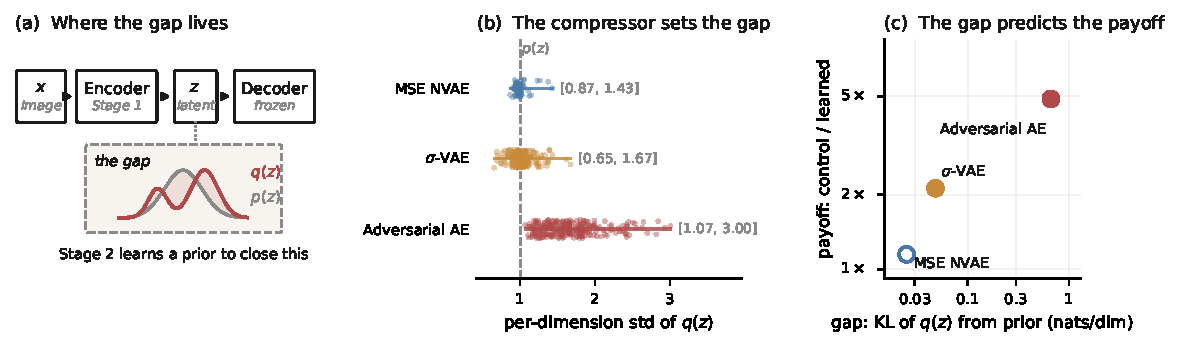
\includegraphics[width=0.96\textwidth]{figures/overview.pdf}
\caption{The argument of this paper in one figure. \textbf{(a)} A two-stage
model freezes a Stage-1 compressor and learns a prior over its latent. The
quantity that decides whether this is worth doing is the gap between the
aggregate posterior $q(z)$ and the prior $p(z)$ the decoder was regularised
toward. \textbf{(b)} That gap is a property of the \emph{compressor}, not of the
prior, and it is measurable before any prior is trained: shown is the
per-dimension standard deviation of $q(z)$ for three Stage-1 objectives on
CelebA $32{\times}32$ (one point per latent dimension). An MSE-trained
hierarchical VAE sits on the prior in overall scale (per-dimension deviations
$[0.87, 1.43]$ about a target of $1$); a perceptual--adversarial
autoencoder, whose KL weight is $10^{-6}$, is nowhere near it
($[1.07, 3.00]$). \textbf{(c)} The gap predicts the payoff. Ordered by the mean
per-dimension KL divergence of $q(z)$ from the prior, the advantage of an
identical learned prior over the best zero-cost closed-form control grows from
$1.15\times$ to $4.9\times$. The open marker is the MSE-trained NVAE, which is
not capacity-matched to the other two (Table~\ref{tab:diagnostic}). Section~\ref{sec:nogap} makes this the paper's
instrument; a handful of points is what we have, and filling in the rest is the
obvious next experiment.}
\label{fig:overview}
\end{figure*}

%======================================================================
\section{Background}
\label{sec:background}

\paragraph{Variational autoencoders.}
A VAE~\cite{vae} pairs an encoder $q_\phi(z\mid x)$ with a decoder
$p_\theta(x\mid z)$ and maximizes the evidence lower bound
\begin{equation}
\mathcal{L} = \mathbb{E}_{q_\phi(z\mid x)}[\log p_\theta(x\mid z)]
              - \beta\, D_{\mathrm{KL}}\!\left(q_\phi(z\mid x)\,\|\,p(z)\right).
\label{eq:elbo}
\end{equation}
Hierarchical variants such as NVAE~\cite{nvae} split $z$ into groups, here a
global vector $\zg$ and a spatial tensor $\zf$, with $\zf$ regularized against
a decoder-predicted conditional prior rather than against $\mathcal{N}(0,I)$.

\paragraph{Latent priors.}
Latent diffusion~\cite{ldm} and LSGM~\cite{lsgm} fit a generative model to the
latent codes of a frozen (or jointly trained) autoencoder. We use two few-step
priors. \emph{Inductive Moment Matching} (IMM)~\cite{imm} trains a map
$f_\psi(z_t,s,t)$ with a kernel moment-matching objective over particle groups.
\emph{MeanFlow}~\cite{meanflow} models the average velocity
$u(z,r,t)=\tfrac{1}{t-r}\int_r^t v(z_\tau,\tau)\,d\tau$ and is trained through
the identity $u = v - (t-r)\,\tfrac{d}{dt}u$, giving one-step sampling
$z_r = z_t - (t-r)u(z_t,r,t)$.

\paragraph{Evaluation.}
We report FID~\cite{fid} throughout with the canonical TF-ported InceptionV3
weights, $50{,}000$ generated samples against $50{,}000$ training images. We
flag this because the protocol matters for the conclusions: an earlier version
of this work used a torchvision ImageNet classifier with $500$--$5{,}000$
samples, which produced internally consistent but non-comparable numbers.

One preprocessing detail matters. Our original CelebA transform resized to
square and then centre-cropped, which makes the crop a no-op and squashes the
$178{\times}218$ frame; we corrected it to \texttt{CenterCrop(148)} followed by
resize. Tables~\ref{tab:oldstack} and~\ref{tab:prdc} (top) retain the
uncorrected models, because what they compare --- priors \emph{within} one
frozen compressor --- is unaffected by the input transform, and their models and
FID reference are consistent with each other.

Table~\ref{tab:diagnostic} compares \emph{across} compressors, so it cannot mix
regimes, and we retrained the MSE-NVAE stack on the corrected crop for it. The
correction is not cosmetic: that stack's free baseline moves from $42.22$ to $155.59$ and its best temperature control from $31.07$ to $104.20$ (at $\sigma=2.2$). We report the corrected
figures and flag that any comparison between the two tables is invalid.

%======================================================================
\section{The diagnostic}
\label{sec:nogap}

\begin{figure*}[t]
\centering
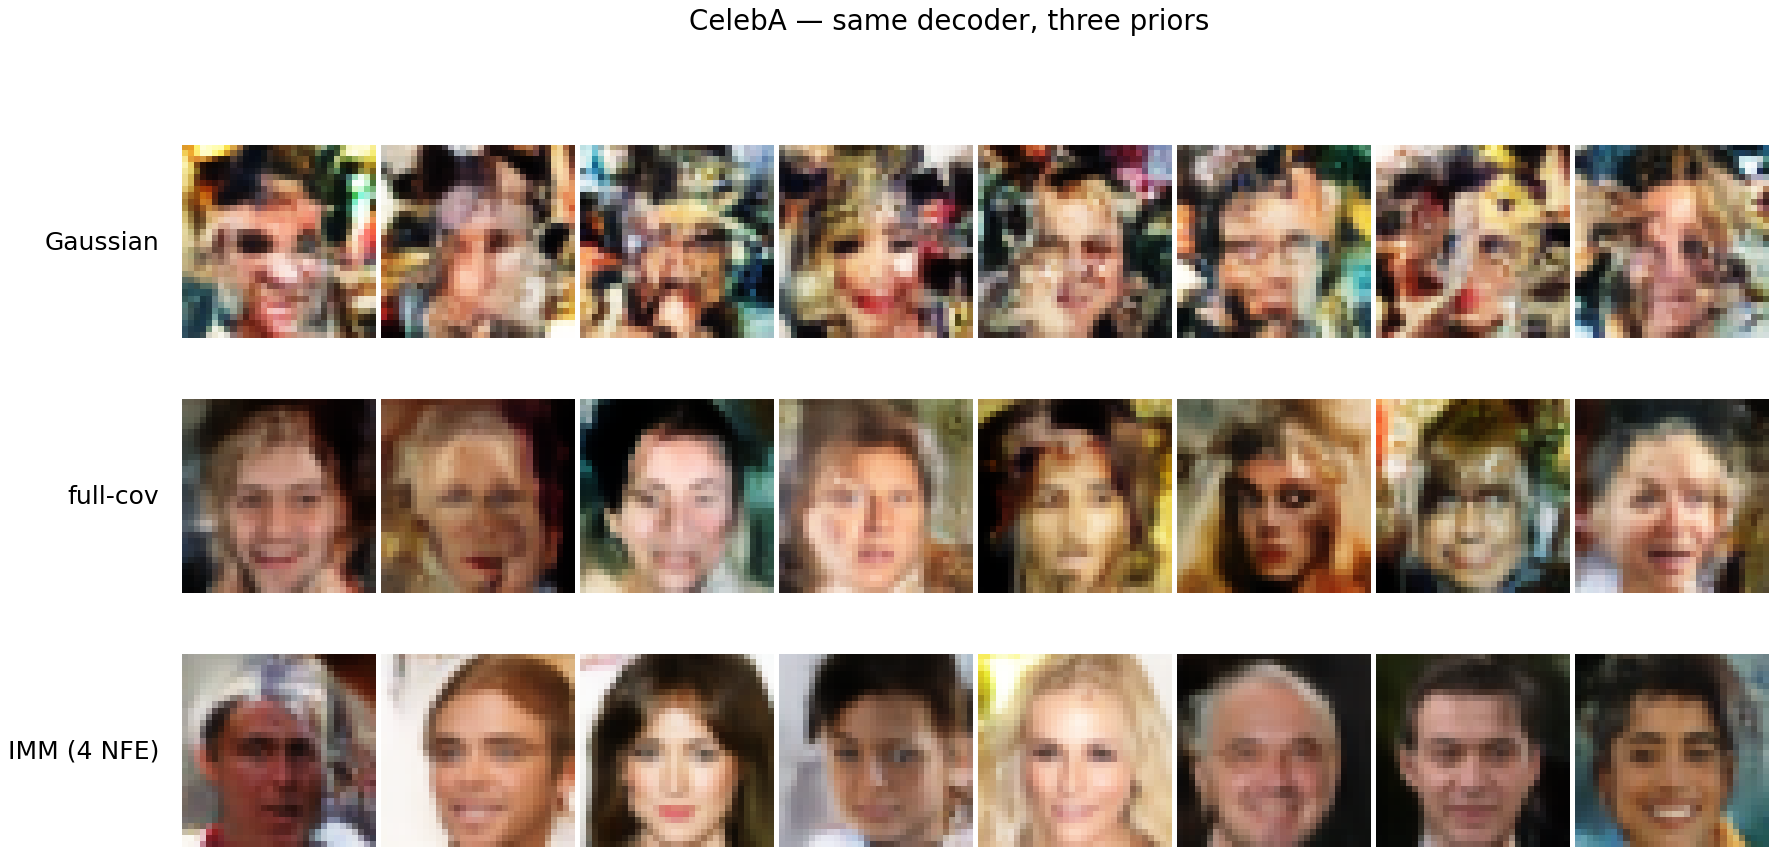
\includegraphics[width=0.86\textwidth]{figures/compare_CelebA.png}
\caption{Qualitative counterpart to the controls in
Table~\ref{tab:main}. CelebA $32{\times}32$, same decoder throughout.
\textbf{Top:} per-dimension Gaussian prior (FID $234.9$).
\textbf{Middle:} full-covariance Gaussian (FID $33.1$) --- recognizable but
soft. \textbf{Bottom:} learned IMM prior at $4$ NFE (FID $6.29$). Most of the
naive Gaussian's failure is missing \emph{correlations}, not scale: the best
temperature-scaled Gaussian still scores $109.30$, while adding the covariance
reaches $33.09$ (Section~\ref{sec:controls}). This is why the covariance control,
not the temperature sweep, is the baseline a learned prior must beat on this
stack.}
\label{fig:compare}
\end{figure*}

Before training any prior, measure $q(z)$. The statistic we use is the
mean, over latent coordinates, of the KL divergence from $\mathcal{N}(0,1)$ of a
Gaussian fitted to that coordinate --- it registers both a shifted mean and a
wrong scale. We also report the FID of each compressor's zero-cost sampler, but
as shown below, that second number is not a reliable measure of the gap.

On the corrected crop (Section~\ref{sec:background}), the MSE-trained
NVAE's $\zg$ has mean $-0.011$ and standard deviation $1.02$, per-dimension
standard deviations in $[0.87, 1.43]$, and a mean per-dimension KL of $0.025$
nats. The model behind Table~\ref{tab:oldstack}, trained before that correction,
gives the same picture: standard deviation $0.98$, per-dimension $[0.96, 1.12]$,
KL $0.003$ nats. In both, the latent sits on the prior --- which is what the
prior-mismatch argument says should not happen. Table~\ref{tab:oldstack} shows
what follows on the original model.

\begin{table}[t]
\caption{MSE-trained NVAE, CelebA $32{\times}32$. Priors over $\zg$. NFE is the
true number of network evaluations. A scalar temperature on the Gaussian prior
beats a $1000$-step diffusion prior, and the best-FID model has the worst
latent fit.}
\label{tab:oldstack}
\begin{tabular}{lrr}
\toprule
Prior over $\zg$ & NFE & FID $\downarrow$ \\
\midrule
Gaussian $\mathcal{N}(0,I)$, KL base      & 0    & 42.22 \\
Gaussian $\mathcal{N}(0,I)$, MMD base     & 0    & 42.06 \\
Temperature $\mathcal{N}(0,1.5^2 I)$      & 0    & \best{31.07} \\
Latent DDPM                               & 1000 & 35.43 \\
MeanFlow                                  & 1    & 40.33 \\
IMM (corrected convention)                & 1    & 32.92 \\
IMM (as originally implemented)           & 16   & 26.37 \\
\bottomrule
\end{tabular}
\end{table}

Two things in Table~\ref{tab:oldstack} are worth stating plainly. First, the
$1000$-step latent DDPM ($35.43$) is \emph{worse} than multiplying Gaussian
samples by $1.5$ ($31.07$). Second, ranking the priors by how well they
reproduce $q(z)$ inverts the FID ranking: MeanFlow attains the best latent
fidelity (kernel MMD $5.1\times10^{-4}$ against held-out encoder latents) and
the worst FID, while the best-FID entry generates latents with standard
deviation $1.61$ against a true $0.98$.

It is tempting to read the second observation as FID being gamed by variance
inflation. Table~\ref{tab:prdc} shows that reading is wrong. Precision, recall,
density and coverage --- $k$-NN manifold estimates rather than a Gaussian fit
--- rank these priors the same way FID does. MeanFlow, the closest match to
$q(z)$, is near-worst on all four; the temperature-scaled Gaussian improves all
four over $\sigma{=}1$ and attains the highest recall of any prior on this
stack. Two independent metrics agree, so the conclusion is not about the
metric. It is that \emph{matching the aggregate posterior is not the right
objective here}: the decoder is not calibrated to $q(z)$ in the way the
prior-mismatch argument assumes, and a prior that deviates from $q(z)$ produces
genuinely better images. What survives is the efficiency comparison --- a free
scalar recovers most of what the learned prior delivers on this compressor.

\begin{table}[t]
\caption{The diagnostic, across five Stage-1 compressors on CelebA
$32{\times}32$. ``Free'' is the FID of that compressor's own zero-cost sampler: a
per-dimension moment-matched Gaussian for the continuous models (not
$\mathcal{N}(0,I)$ --- the empirical per-dimension mean and standard deviation
are used, which is the stronger baseline), ancestral sampling at $t{=}1$ for the
NVAE, independent marginal codes for VQ. ``Control'' is the best closed-form
prior of Section~\ref{sec:controls} where one exists; the VQ codebook has no
covariance analogue, and the NVAE's is its temperature-swept ancestral sampler
with recalibrated BatchNorm statistics (Section~\ref{sec:nvae}). Gain is
control\,/\,learned. $^\ddagger$VQ has no closed-form control, so its gain is
free\,/\,learned and is not comparable to the other rows: measured the same way,
the perceptual--adversarial autoencoder's would also be $37\times$. $^\dagger$The MSE-NVAE row is not capacity-matched to the
others: its latent is $8256$-dimensional against $256$, and its free sampler
draws only the $64$-dimensional $\zg$ while the decoder's own conditional prior
supplies the remaining $8192$. Its free FID therefore measures a different
object than the single-level rows and should not be read as a point on a ladder
with them; we retain the row because its \emph{within-compressor} comparison
(Table~\ref{tab:oldstack}) is the paper's opening result. Its Stage-2 prior was retrained
under the corrected crop for the same $100$ epochs as the original. The Free and Ceiling columns are measured before Stage~2 and
are what the diagnostic uses; Learned and Gain are Stage-2 outcomes and are what
it is tested against.}
\label{tab:diagnostic}
\small
\begin{tabular}{lrrrrr}
\toprule
Stage-1 compressor & Free & Control & Learned & Gain & Ceiling \\
\midrule
MSE NVAE ($\zg$)$^\dagger$ & 155.59 & 104.20 & 90.71 & $1.15\times$ & 1.67 \\
Proper NVAE (matched)     & 75.83  & 44.13 & ---   & ---         & 11.79 \\
$\sigma$-VAE              & 109.49 & 29.62 & 13.94 & $2.1\times$ & 9.41 \\
VQ-VAE (EMA codebook)     & 244.74 & ---   & 6.57  & $37\times^\ddagger$ & 3.48 \\
Perceptual--adversarial   & 234.87 & 30.74 & \best{6.29}  & \best{$4.9\times$} & \best{2.01} \\
\bottomrule
\end{tabular}
\end{table}

\paragraph{The diagnostic predicts the payoff.}
Table~\ref{tab:diagnostic} is the paper's instrument. Three of its rows
carry both a closed-form control and a learned prior, so they can test it.
Ordered by how far each aggregate posterior sits from the prior --- mean
per-dimension KL $0.025$, $0.048$ and $0.664$ nats for the MSE-NVAE, the
$\sigma$-VAE and the adversarial autoencoder --- the gains follow: $1.15\times$,
$2.1\times$ and $4.9\times$. The mean per-dimension standard deviation, the
statistic we first reached for, does not separate the first two ($1.00$ vs.\
$1.01$), because it ignores mean offsets and averages out spread across
coordinates. The MSE-NVAE row is not capacity-matched to the other two (see the
table's footnote), so this is three points, one of them qualified.
VQ, whose discrete latent has no Gaussian to match at all, recovers almost the
entire distance to its ceiling. That ordering is the paper's claim, and it is
measured before any Stage-2 prior is trained.

One column does \emph{not} order this way, and we flag it because it is the
obvious thing to reach for. Across the MSE-NVAE, $\sigma$-VAE, VQ and adversarial rows,
free FID spans only $2.2\times$, and the MSE-NVAE's free baseline ($156$) is worse than the $\sigma$-VAE's ($109$) even though its aggregate
posterior is closer to the prior. Free FID confounds the size of the gap with
how sharply a decoder degrades off its training distribution, so the diagnostic
we propose is the KL statistic above, not the free baseline. The $\sigma$-VAE is the informative middle case: by
calibrating the observation variance rather than fixing $\beta$, it applies a
far stronger effective KL than the adversarial autoencoder, which pulls $q(z)$
back toward the prior --- and its learned prior correspondingly buys less.

Two cautions follow from the same table. First, the gap is not a proxy for
quality: the $\sigma$-VAE and the adversarial autoencoder have best
controls within $29.6$--$30.7$, yet their ceilings differ by $4.7\times$
($9.41$ vs.\ $2.01$). A large
gap means a prior has room to work, not that the resulting samples will be good.
Second, the ranking by gain is not the ranking by FID --- the $\sigma$-VAE's
learned prior reaches $13.94$ against a ceiling of $9.41$, closer to its own
ceiling ($1.5\times$) than the adversarial stack is to its own ($3.1\times$).

The proper NVAE is the row that most sharply separates the two axes, and it
contradicts the prediction its architecture invites. Because its prior is
conditional and trained jointly with the encoder, ancestral sampling already is
a learned hierarchical prior, so one expects the gap to be closed by
construction. It is not: at matched capacity, ancestral sampling at its best temperature
reaches $44.13$ against a ceiling of $11.79$, a $3.7\times$ shortfall. Joint training of a conditional prior
does not by itself make that prior match the aggregate posterior.

We initially read a much larger shortfall ($25\times$) as evidence about the
training objective, but that model was $7\times$ over-complete and the reading
does not survive matching capacity (Section~\ref{sec:nvae}). What the row
supports is narrower and still useful: the hierarchy is the one compressor whose
prior is learned \emph{during} Stage 1, and it is also the one where a
second-stage prior cannot help --- for a reason we identify in
Section~\ref{sec:nvae}.

The VQ row reaches essentially the same FID as the adversarial autoencoder
($6.57$ vs.\ $6.29$) from a far worse free baseline ($244.74$ vs.\ $234.87$),
giving the largest gain in the table. A discrete latent has no Gaussian to
mismatch, so the naive baseline --- independent codes drawn from their marginal
frequencies --- is very weak, and almost the entire distance to the ceiling is
recoverable by a prior that models the joint: VQ's prior closes $98.7\%$ of
the distance from its free baseline to its ceiling. That figure is not
comparable to the headroom column of Table~\ref{tab:main}, which is measured
from the strongest closed-form control; measured from the free baseline as VQ's
is, the adversarial autoencoder closes $98.2\%$ and the $\sigma$-VAE $95.5\%$.
What sets VQ apart is only that it has no closed-form control to beat. Appendix~\ref{app:vq} reports the codebook repair this depends on, and a
sampler bug that inverted the conclusion before we caught it.

%======================================================================
\section{Controls}
\label{sec:controls}

Because a naive Gaussian is a weak baseline, we benchmark against three
closed-form priors, all requiring zero network evaluations. Let $\mu$ and
$\Sigma$ be the mean and covariance of the training latents and
$\Sigma = LL^\top$.

\begin{enumerate}
\item \textbf{Temperature.} $z = \mu + \sigma\,\mathrm{diag}(s)\,\epsilon$,
sweeping $\sigma$. Detects gains that are only rescaling.
\item \textbf{Full covariance.} $z = \mu + L\epsilon$. Detects gains that are
only second-order correlations.
\item \textbf{Copula.} Whiten to $u = L^{-1}(z-\mu)$, then match each
coordinate's empirical marginal by an inverse-CDF transform of a Gaussian
sample. Adds exact per-dimension marginals on top of the covariance.
\end{enumerate}

These are not straw men. On the MSE stack the temperature control beats every
learned prior we trained except one; on a compressed variant of that stack the
covariance-plus-copula control ($40.97$) beat a conv-architecture MeanFlow
prior trained for $150$ epochs ($45.66$). A learned prior that does not clear
these baselines is not demonstrating prior expressivity.

The three controls also separate \emph{which} deficiency of the naive Gaussian
matters, and the answer differs by stack. On the adversarial autoencoder,
sweeping the temperature of a per-dimension Gaussian improves FID from $234.62$
at $\sigma{=}1$ to $109.30$ at $\sigma{=}0.5$ --- a real gain, and still $3.3\times$
worse than simply adding the covariance ($33.09$). Getting the scale right is
therefore worth much less here than getting the correlations right, which is
what Figure~\ref{fig:compare} shows qualitatively. On the MSE stack the temperature
control is the strongest closed-form prior we evaluated, but we did not run a
covariance control over its $\zg$, so we cannot say whether correlations matter
less there. On a compressed variant of that stack, adding a covariance over
$\zf$ did help substantially ($55.1 \to 39.5$).

%======================================================================
\section{Method}
\label{sec:method}

\paragraph{Stage 1.}
Following~\cite{ldm}, we train an autoencoder with an $L_1$ reconstruction
term, an LPIPS perceptual term~\cite{lpips}, a PatchGAN adversarial
term~\cite{patchgan} with the adaptive weighting of~\cite{ldm}, and a
negligible KL weight ($10^{-6}$). The latent is $\tfrac{S}{4}\times
\tfrac{S}{4}\times 4$ for an $S\times S$ image, so the compression ratio
($0.083\times$) is held fixed across resolutions.

\paragraph{Stage 2.}
Stage 1 is frozen and latents are extracted once. The prior is a convolutional
residual network over the latent grid (4.64M parameters), trained with either
the IMM objective or the MeanFlow identity. Architecture, width, depth,
learning rate and schedule are identical across all datasets and resolutions.

\paragraph{Corrections.}
Three implementation errors materially affected our earlier results and are
documented here for reproducibility. (i) MeanFlow's identity differentiates
through the time embedding with respect to $t$; scaling the embedding input by
$1000$, as is standard in diffusion networks that never take this derivative,
makes $\partial\,\mathrm{emb}/\partial t$ up to $1000\times$ too large and the
regression target is swamped. With the scale at $1$ the model recovers an
8-mode ring (excess kurtosis $-1.40$ against a true $-1.47$); at $1000$ it
returns Gaussian output ($-0.01$). (ii) The IMM implementation interpolated
$x_t = t x + (1-t)\epsilon$, placing data at $t{=}1$, while drawing $s<t$ as if
data were at $t{=}0$; the learned map is then a noising map. On the ring, the
uncorrected convention gives radius std $1.46$ against a true $0.11$. (iii) The
sampler applied each transition twice, so reported step counts understated NFE
by $2\times$. (iv) Our FID cache was keyed on (backbone, prior, NFE) but not on
model capacity or protocol, so re-running a configuration after retraining its
prior silently returned the previous model's row. We widened the key and
recomputed every affected entry. The recomputation is self-checking: on LSUN and
ImageNet-32 all ten cached rows reproduced exactly ($\Delta = 0.000$), which
establishes that sampling and scoring are deterministic here, so the shifts of
up to $0.50$ FID on CelebA and FFHQ are attributable to a changed checkpoint
rather than to sampler noise. All reported values are the recomputed ones. (v) The corrected-crop
Stage-2 prior of Table~\ref{tab:diagnostic} was first trained by a run that the
operating system killed for memory pressure partway through. That checkpoint
gave FID $128.53$, a gain of $0.81\times$ --- i.e.\ it
suggested the learned prior \emph{loses} to a scalar temperature on this
compressor. Trained to its full $100$ epochs the same configuration reaches $90.71$ ($1.15\times$). We record this because
the interrupted number was self-consistent and would have supported a striking
claim; only the budget was wrong.

%======================================================================
\section{Results}
\label{sec:results}

\begin{table*}[t]
\caption{Main result. Standard-protocol FID ($50$k vs.\ $50$k, canonical
Inception). All rows share one Stage-1 protocol and one Stage-2
architecture, with no per-dataset tuning. ``Ceiling'' decodes ground-truth
encoder latents and bounds what any prior can achieve. Gain is best
closed-form control divided by best learned prior. Learned-prior entries are
mean $\pm$ standard deviation over three sampling seeds. Headroom is
$(\text{control} - \text{achieved}) / (\text{control} - \text{ceiling})$: the
fraction of the available improvement the prior actually captures. Raw FID
varies $12\times$ across these settings and headroom varies $1.4\times$, so it
is headroom that is comparable across datasets.}
\label{tab:main}
\begin{tabular}{llrrrrrrrr}
\toprule
& & \multicolumn{3}{c}{Closed-form controls (0 NFE)} & \multicolumn{2}{c}{Learned prior} & & \\
\cmidrule(lr){3-5}\cmidrule(lr){6-7}
Dataset & Res. & Gaussian & Full-cov. & Copula & FID & NFE & Ceiling & Gain & Headroom \\
\midrule
CelebA      & 32 & 234.90 & 33.09  & 30.74  & \best{6.29}\std{0.04}  & 4  & 2.01  & $4.9\times$ & \best{0.85} \\
FFHQ        & 32 & 242.14 & 37.81  & 36.79  & \best{15.16}\std{0.04} & 2  & 5.49  & $2.4\times$ & 0.69 \\
CelebA      & 64 & 318.57 & 65.62  & 63.52  & \best{23.35}\std{0.07} & 4  & 2.19  & $2.7\times$ & 0.66 \\
LSUN church & 32 & 152.58 & 79.01  & 77.29  & \best{22.79}\std{0.12} & 4  & 7.58  & $3.4\times$ & 0.78 \\
CIFAR-10    & 32 & 183.10 & 95.24  & 93.45  & \best{45.95}\std{0.09} & 4  & 15.33 & $2.0\times$ & 0.61 \\
ImageNet-32 & 32 & 210.43 & 127.85 & 126.64 & \best{75.74}\std{0.27} & 16 & 42.67 & $1.7\times$ & 0.61 \\
\bottomrule
\end{tabular}
\end{table*}

Table~\ref{tab:main} is the main result. On all six settings the learned prior
clears all three closed-form controls, by $1.7$--$4.9\times$, against
$1.15\times$ on the MSE stack. Because the ceilings span $2.01$ to $42.67$, raw FID is not comparable
across datasets and we report headroom alongside it: the prior captures
$61$--$85\%$ of the improvement its compressor makes available, everywhere. That
single range is the claim; the FID column is the detail behind it. Note also
that the two orderings differ --- LSUN is fourth on raw FID and second on
headroom --- so a dataset can look weak in absolute terms while its prior is
doing well against what the compressor allows. Figure~\ref{fig:compare} shows the same progression qualitatively.

\paragraph{The gain is largest where the data is easiest, but not monotonically
so.}
The extremes are ordered as the story predicts --- $4.9\times$ on aligned CelebA
faces, $1.7\times$ on ImageNet-32 --- and we report this rather than only the
strongest dataset, because the ``expressive prior'' case is strongest exactly
where the data is easiest. The middle of the range is \emph{not} ordered by
domain, however, and we state that rather than presenting a subset that is:
FFHQ is aligned faces yet gains less than LSUN scenes ($2.4\times$ vs.\
$3.4\times$). Resolution moves the gain as much as domain does --- the same
CelebA data at $64{\times}64$ falls from $4.9\times$ to $2.7\times$ --- so
``difficulty'' here confounds domain diversity with latent dimension, and we
cannot separate the two with six settings. On ImageNet-32 the binding constraint is Stage 1, not the
prior --- decoding ground-truth latents already gives FID $42.67$, so a
$12$M-parameter autoencoder at $0.083\times$ compression cannot represent
$1000$-class ImageNet, and the prior recovers most of the headroom that
remains ($210 \rightarrow 76$).

\paragraph{Resolution.}
Moving CelebA from $32$ to $64$ at fixed compression ratio barely changes the
ceiling ($2.01 \to 2.19$) but widens the prior's gap to it ($3.1\times \to
10.7\times$). The latent's excess kurtosis rises from $+0.23$ to $+1.28$ over
the same change: four times the latent dimension yields a substantially more
non-Gaussian target that the same $4.64$M prior cannot match. At higher
resolution the prior, not the autoencoder, is the binding constraint.

\begin{table}[t]
\caption{Precision / recall / density / coverage, $k{=}5$, $10$k vs.\ $10$k on
the same Inception features used for FID. \textbf{Top:} the MSE stack --- all
four metrics rank the priors as FID does, so the ranking is not a FID artifact,
and the free temperature control attains the best recall. \textbf{Bottom:} the
adversarial stack on all six settings. The learned prior's advantage is
\emph{diversity}: recall spans $0.007$--$0.171$ for the closed-form control and
$0.140$--$0.535$ for the learned prior, with no overlap, while precision is
lower for the learned prior on CIFAR-10 and ImageNet-32. Reporting CelebA alone
would have suggested it wins on every axis.}
\label{tab:prdc}
\small
\begin{tabular}{llrrrr}
\toprule
Dataset & Prior & P $\uparrow$ & R $\uparrow$ & D $\uparrow$ & C $\uparrow$ \\
\midrule
\multicolumn{6}{l}{\emph{MSE-trained NVAE, CelebA $32$}}\\
& Gaussian $\sigma{=}1.0$ (FID 42.2)    & 0.312 & 0.261 & 0.124 & 0.163 \\
& Temperature $\sigma{=}1.5$ (FID 31.1) & 0.357 & \best{0.425} & 0.146 & 0.206 \\
& IMM-legacy (FID 26.4)                 & \best{0.413} & 0.388 & \best{0.186} & \best{0.259} \\
& MeanFlow, best latent fit (FID 40.3)  & 0.333 & 0.244 & 0.137 & 0.179 \\
\midrule
\multicolumn{6}{l}{\emph{Perceptual--adversarial autoencoder}}\\
\multirow{2}{*}{CelebA 32}   & full-cov & 0.783 & 0.171 & 0.734 & 0.378 \\
                             & IMM      & \best{0.837} & \best{0.535} & \best{1.336} & \best{0.918} \\
\multirow{2}{*}{FFHQ 32}     & full-cov & 0.750 & 0.113 & 0.884 & 0.467 \\
                             & IMM      & \best{0.791} & \best{0.414} & \best{1.226} & \best{0.815} \\
\multirow{2}{*}{CelebA 64}   & full-cov & 0.542 & 0.007 & 0.277 & 0.106 \\
                             & IMM      & \best{0.718} & \best{0.264} & \best{0.786} & \best{0.575} \\
\multirow{2}{*}{LSUN 32}     & full-cov & 0.614 & 0.071 & 0.434 & 0.212 \\
                             & IMM      & \best{0.656} & \best{0.375} & \best{0.763} & \best{0.692} \\
\multirow{2}{*}{CIFAR-10}    & full-cov & \best{0.692} & 0.050 & 0.515 & 0.148 \\
                             & IMM      & 0.662 & \best{0.433} & \best{0.567} & \best{0.342} \\
\multirow{2}{*}{ImageNet-32} & full-cov & \best{0.668} & 0.007 & \best{0.559} & 0.168 \\
                             & IMM      & 0.594 & \best{0.140} & 0.448 & \best{0.315} \\
\bottomrule
\end{tabular}
\end{table}

\paragraph{The gain is in coverage, not fidelity.}
Table~\ref{tab:prdc} separates the two axes FID conflates, and the separation is
consistent across all six settings. The covariance control produces individually
plausible samples --- precision $0.54$--$0.78$, visible in
Figure~\ref{fig:compare} as faces that are recognisable but similar --- while
covering $11$--$47\%$ of the real manifold. The learned prior covers
$32$--$92\%$. On CIFAR-10 and ImageNet-32 it is in fact \emph{less} precise than
the control ($0.662$ vs.\ $0.692$; $0.594$ vs.\ $0.668$) and still far better
overall, because recall improves by $8.7\times$ and $20\times$. Diversity is
what a Gaussian baseline cannot buy at any temperature, and it is what the
learned prior supplies.

\begin{figure}[t]
\centering
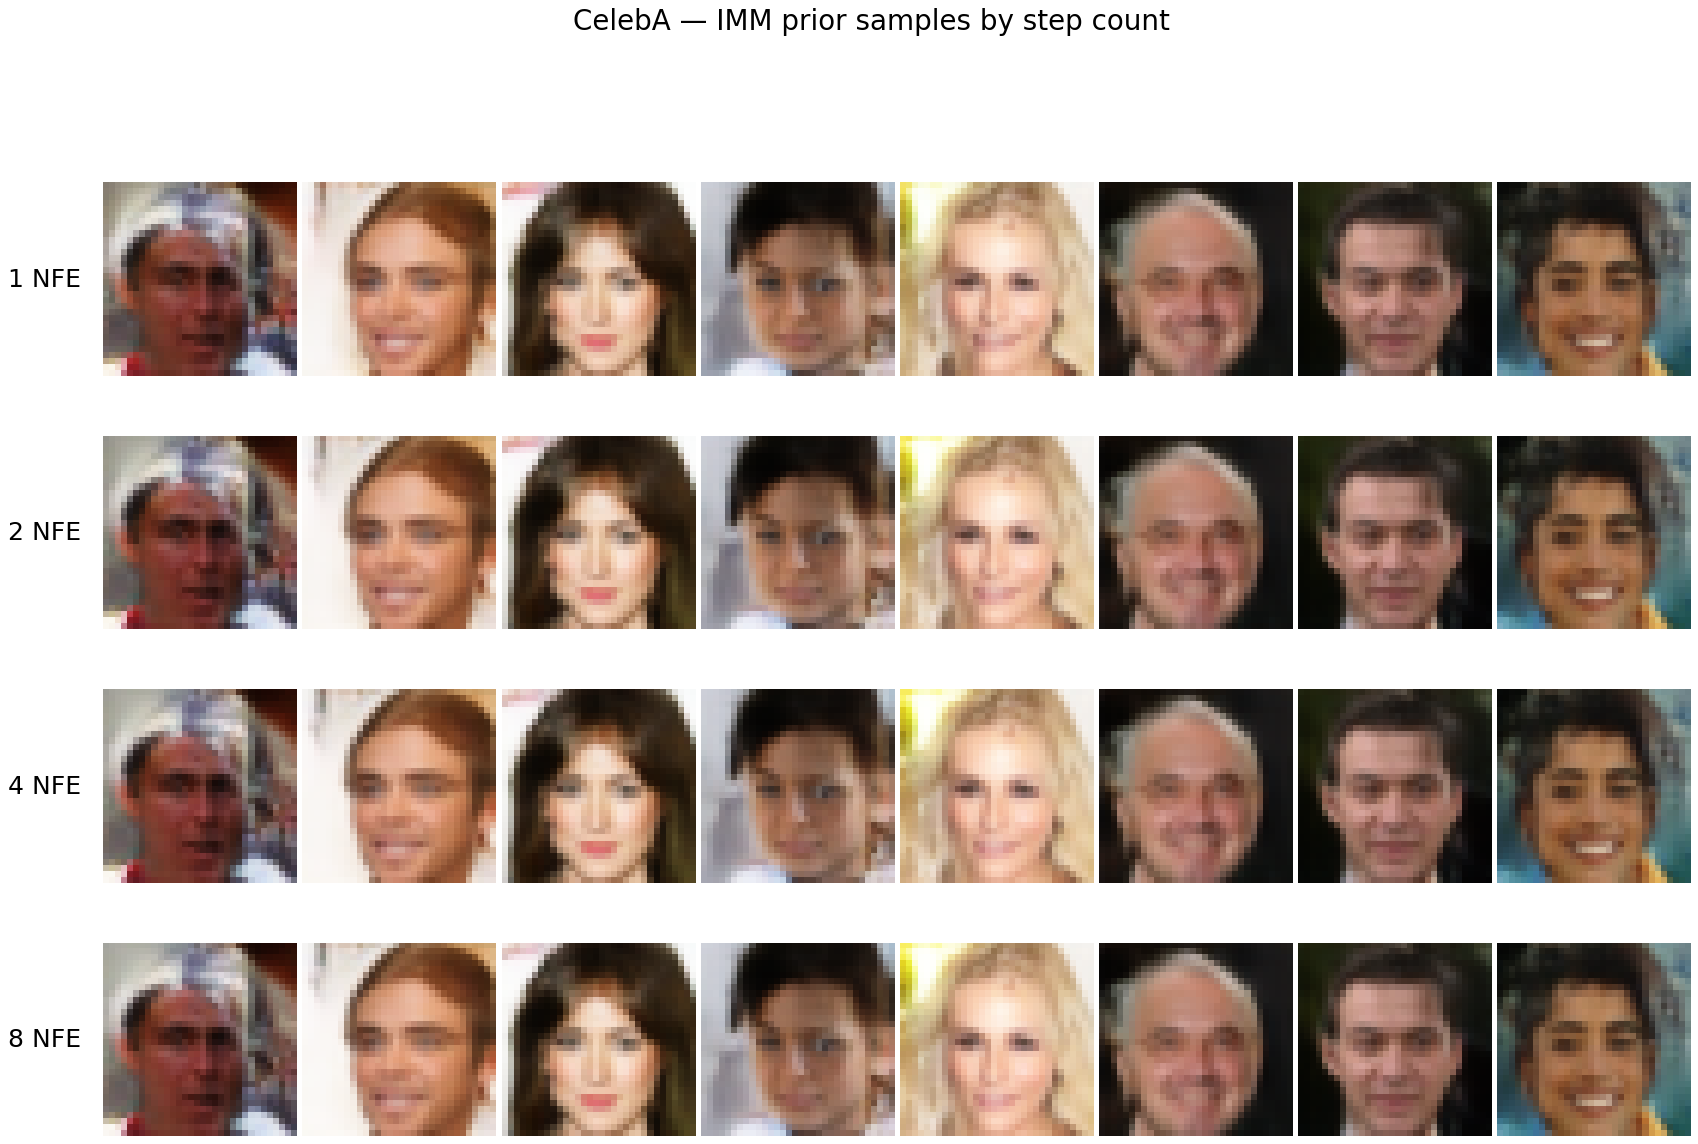
\includegraphics[width=\columnwidth]{figures/samples_CelebA.png}
\caption{IMM prior samples on CelebA $32{\times}32$ by step count. Quality
changes little from 2 to 8 NFE (FID $6.40$--$6.36$, Table~\ref{tab:nfe}); a
single evaluation costs about $1.2$ FID ($7.47$).}
\label{fig:samples}
\end{figure}

\begin{table}[t]
\caption{IMM versus MeanFlow at matched NFE, identical conv trunk ($4.64$M
parameters), budget and schedule. IMM wins in every cell, and MeanFlow degrades
past $1$--$2$ NFE on all four datasets. Single sampling seed; the three-seed
means for the best configurations are in Table~\ref{tab:main}.}
\label{tab:nfe}
\small
\begin{tabular}{llrrrr}
\toprule
Dataset & Prior & 1 & 2 & 4 & 8 \\
\midrule
\multirow{2}{*}{CelebA} & IMM & \best{7.47} & \best{6.40} & \best{6.25} & \best{6.36} \\
                          & MeanFlow & 13.44 & 12.59 & 14.13 & 14.96 \\
\midrule
\multirow{2}{*}{FFHQ} & IMM & \best{16.90} & \best{15.13} & \best{15.59} & \best{16.23} \\
                          & MeanFlow & 26.27 & 27.02 & 28.83 & 29.92 \\
\midrule
\multirow{2}{*}{LSUN} & IMM & \best{24.83} & \best{23.13} & \best{22.82} & \best{23.20} \\
                          & MeanFlow & 33.74 & 33.71 & 35.38 & 36.36 \\
\midrule
\multirow{2}{*}{CIFAR-10} & IMM & \best{48.33} & \best{46.21} & \best{45.86} & \best{46.05} \\
                          & MeanFlow & 66.02 & 65.96 & 67.88 & 69.15 \\
\bottomrule
\end{tabular}
\end{table}

\paragraph{IMM outperforms MeanFlow, with a mechanism.}
Table~\ref{tab:nfe} shows IMM ahead at every step count on all four datasets
we ran both methods on, by $1.4$--$2.0\times$ at each method's own best NFE. MeanFlow additionally
degrades past $1$--$2$ NFE on every dataset, which we attribute to its
objective rather than to tuning: MeanFlow regresses onto a conditional mean, and iterating that map
compounds the bias. Two measurements support this. Spatial autocorrelation
within each latent channel rises monotonically with NFE and overshoots the
true value ($0.293 \to 0.313$ against $0.305$), i.e.\ samples become
progressively over-smoothed; and the covariance error is minimized at exactly
the NFE that minimizes FID. IMM's objective is distributional rather than a
pointwise regression and shows no such degradation.

\paragraph{Efficiency, timed.}
NFE is not by itself an efficiency measure --- a step of a $4.64$M-parameter CNN
is not a step of a 6-block MLP --- so we time the samplers
(Appendix~\ref{app:support}, Table~\ref{tab:time}). Our best configuration
samples in $174.6$\,ms per $1000$ images against $6063.7$\,ms for the
$1000$-step latent DDPM, a $35\times$ difference in time alongside the
difference in quality. The comparison that does \emph{not} favour us is against
the closed-form control: at $65.8$\,ms it is only $2.7\times$ faster than the
learned prior, because decoding dominates once the prior is cheap. The learned
prior's case rests on quality (Tables~\ref{tab:main},~\ref{tab:prdc}), not on
being fast relative to a matrix multiply.

\paragraph{Reconstruction, conventionally measured.}
Among capacity-matched compressors the reconstruction ordering follows the
training objective rather than the generative ranking: the $\sigma$-VAE leads on
PSNR/SSIM, the adversarial autoencoder on LPIPS, and quantisation costs VQ about
$3$\,dB (Appendix~\ref{app:support}, Table~\ref{tab:recon}). None of these
orderings predicts the Gain column of Table~\ref{tab:diagnostic}, which is the
point: how well a compressor reconstructs and how much room it leaves a prior
are different questions.

%======================================================================
\section{Does this transfer to hierarchical models?}
\label{sec:nvae}

Everything so far concerns a single-level latent, where Stage 2 replaces one
fixed prior. Hierarchical VAEs already have a learned, jointly-trained
conditional prior for every group, so they are the natural stress test: if the
gap can be closed architecturally, it should be closed here. We built a proper
NVAE --- bidirectional inference, residual normal posteriors, per-group
conditional priors, KL warm-up, per-dimension free bits --- with six latent
groups over three scales.

\begin{table}[t]
\caption{Proper NVAE on CelebA $32{\times}32$, at matched latent capacity and
at $7\times$ over-complete. Capacity, not architecture, is what produces the
striking ceiling: at the same $256$-dimensional budget as every other
compressor in Table~\ref{tab:diagnostic}, the hierarchy reconstructs far worse
than any of them.}
\label{tab:nvae}
\small
\begin{tabular}{lrr}
\toprule
 & Matched & Over-complete \\
 & 256 dims & 21{,}504 dims \\
 & ($0.083\times$) & ($7\times$) \\
\midrule
Posterior reconstructions (ceiling) & 11.79 & \best{2.01} \\
Ancestral sampling, $t{=}1.0$       & 75.83 & 144.82 \\
Ancestral sampling, $t{=}0.8$       & 63.37 & 74.52 \\
\;\;+ BN recalibrated, $t{=}1.0$    & 67.18 & 68.04 \\
\;\;+ BN recalibrated, $t{=}0.8$    & 47.59 & 51.31 \\
\;\;+ BN recalibrated, best $t$ tested & \best{44.13} ($t{=}0.6$) & 50.76 ($t{=}0.7$) \\
Gap (best sampling / ceiling)       & $3.7\times$ & $25\times$ \\
\midrule
\multicolumn{3}{l}{\emph{+ scheduled sampling ($p{=}0.3$)}}\\
\;\;Reconstructions (ceiling)               & 13.01 & --- \\
\;\;Ancestral at own optimum $t{=}0.9$      & \best{40.88} & --- \\
\;\;Gap (best sampling / ceiling)           & $3.1\times$ & --- \\
\bottomrule
\end{tabular}
\end{table}

\paragraph{At matched capacity the hierarchy is simply a worse compressor.}
Our first NVAE used six groups of eight channels across three scales, which is
$21{,}504$ latent dimensions for a $3{,}072$-dimensional image --- $7\times$
over-complete, and $84\times$ the budget of every other compressor we compare
against. It reconstructs almost losslessly (PSNR $44.0$\,dB, LPIPS $0.0001$) and
reaches a ceiling of $2.01$, matching the adversarial autoencoder. That match is
capacity, not architecture. Constraining the hierarchy to the same $256$
dimensions --- four groups at the coarsest scale, since a single group at full
resolution already costs $1024$ dimensions --- moves the ceiling to $11.79$,
worse than the adversarial autoencoder ($2.01$), the $\sigma$-VAE ($9.41$) and
both VQ variants ($3.48$, $3.90$).

This is the same pathology we identify in the prior work of
Section~\ref{sec:intro}, and we reproduced it before catching it: an
over-complete hierarchical latent buys reconstruction that a compressive one
cannot, and reporting the resulting ceiling as an architectural property is a
mistake in either direction.

\paragraph{One large loss is an implementation defect, not a modelling one.}
NVAE's cells use BatchNorm, whose running statistics are accumulated while
activations are driven by \emph{posterior} samples. Ancestral sampling drives
them differently, so the stored statistics are wrong exactly when generating.
Re-estimating them from $20$k prior samples --- no training --- recovers
$63.37 \to 47.59$ at matched capacity and $74.52 \to 51.31$ on the
over-complete model (both at $t{=}0.8$; at $t{=}1.0$ the over-complete model goes $144.82 \to 68.04$). The effect replicates across both, so it is a defect in the
implementation rather than an artifact of over-parameterisation. Replacing
BatchNorm with GroupNorm removes the mechanism entirely and gives a ceiling of $1.67$,
among the best we measured, but cannot recover as much, because GroupNorm has
no statistics to correct. We report both because the distinction matters: one
repairs a defect, the other prevents it. Together with a temperature search,
these implementation-level fixes close most of the sampling gap with no training
and no new parameters, while both Stage-2 priors we tried made it worse.

\begin{table}[t]
\caption{Mixed sampling on the six-group hierarchy: groups $1..k$ from the
prior, the rest from the posterior of a held-out image. The loss is not
distributed --- the three coarsest groups are free, and everything breaks at the
fine-scale groups.}
\label{tab:mixed}
\small
\begin{tabular}{lrrrrrrr}
\toprule
$k$ (groups from prior) & 0 & 1 & 2 & 3 & 4 & 5 & 6 \\
\midrule
FID & 3.11 & 2.96 & 2.68 & \best{2.56} & 29.65 & 90.17 & 144.35 \\
\bottomrule
\end{tabular}
\end{table}

\paragraph{Damping is needed everywhere, not only where the loss appears.}
Table~\ref{tab:mixed} suggests the coarse groups are harmless, so we expected a
schedule that damps only groups 4--6 to beat a uniform one. It does not:
holding the coarse groups at $t{=}1$ and damping the fine groups to
$0.6$--$0.8$ gives $53.5$--$59.4$, against $50.76$ for a uniform $t{=}0.7$. The
sweep measures each group with \emph{later groups drawn from the posterior};
under full ancestral sampling a coarse group's variance also propagates into
every later group's conditioning. A group can be individually harmless and
still need damping for what it does downstream.

\paragraph{The residual gap is not reachable by a second-stage prior.}
The remaining experiments in this section were run on the over-complete model,
where the gap is largest and therefore easiest to attribute; we have not
repeated them at matched capacity. Table~\ref{tab:mixed} localises it: sampling the three coarsest groups from the
prior costs nothing, and the two $32{\times}32$ groups cost everything. We
tested Stage-2 priors in both places. On group~1 --- which the sweep shows is
already free, and whose aggregate posterior is nearly its prior (std $0.687$,
excess kurtosis $+0.124$) --- an IMM prior fits well (latent MMD $4.2\times
10^{-4}$) and changes nothing ($74.5 \to 80.0$). On groups 4--6, conditioned on
the top-down state and parameterised residually so that $\epsilon \sim
\mathcal{N}(0,I)$ reproduces NVAE's own conditional Gaussian exactly, the priors
are actively harmful ($78.6 \to 95.8$) and their loss flatlines after six
epochs.

We read this as exposure bias rather than prior capacity. Each conditional prior
is trained on contexts $z_{<l}$ drawn from the posterior, but at sampling time
$z_{<l}$ comes from the prior. By group~4 the context has drifted off the
posterior manifold, so every downstream conditional is evaluated out of
distribution --- and a prior fitted on posterior-derived $(h_l, \epsilon_l)$
pairs cannot help, because those are not the pairs it meets at sampling time.

\paragraph{Fixing the contexts, not the prior, is what works.}
That diagnosis makes a prediction: an intervention that changes \emph{which
contexts the model is trained on} should succeed where better priors on the old
contexts failed. We fine-tune the hierarchy with scheduled sampling, replacing
each group's context with a draw from its own prior with probability
$p{=}0.3$, keeping the real image as the reconstruction target. This is the only
one of our three interventions that helps. Fine-tuning on partly sampled
contexts moves the temperature optimum, so the like-for-like comparison is each
model at its own best temperature (Table~\ref{tab:temp}): $44.13$ at
$t{=}0.6$ against $40.88$ at $t{=}0.9$, a $7.4\%$ improvement, at a cost of
$1.2$ FID on the ceiling ($11.79 \to 13.01$) --- the trade the method predicts,
since reconstructing from a partly sampled context is genuinely harder.

\begin{table}[h]
\caption{Three interventions on the same hierarchy. Only the one that changes
the training contexts helps.}
\small
\begin{tabular}{lr}
\toprule
Intervention & FID \\
\midrule
Stage-2 prior on group 1 (over-complete)     & $74.5 \to 80.0$ \\
Stage-2 priors on groups 4--6 (over-complete)& $78.6 \to 95.8$ \\
Scheduled sampling (matched)                 & $44.1 \to \best{40.9}$ \\
\bottomrule
\end{tabular}
\end{table}

So the earlier negatives are not evidence that hierarchical sampling gaps are
unreachable; they are evidence that \emph{post-hoc} priors cannot reach them.
The gap is created during training and has to be addressed there.

\paragraph{The intervention moves the optimum, not the sensitivity.}
The clearest signature is where each model wants its temperature.
Table~\ref{tab:temp} sweeps $t$ for both. The baseline is best at $t{=}0.6$:
it must have its own prior samples shrunk to look good, which is what a model
that cannot handle those samples does. After fine-tuning the optimum moves to
$t{=}0.9$, near full prior variance. That shift is the exposure-bias
prediction, and it is why the two models must be compared at their own optima
rather than at a shared $t$.

What does \emph{not} change is how sharply either model depends on temperature:
both stay within $10\%$ of their optimum over a $t$-window of width $0.34$. We
report this because our first reading of these curves was that scheduled
sampling had flattened them, which came from sweeping only $t \in [0.6, 1.0]$ ---
a range that straddles the baseline's optimum but sits at the edge of the
fine-tuned model's. Widening the grid removed the effect. The intervention
relocates the optimum; it does not make the model robust to a mis-set
temperature.

\paragraph{What temperature sensitivity measures.}
Steepness invites a general reading --- that a sharp temperature optimum
indicates train/test context mismatch. A control settles it. We sweep the same
temperature on two \emph{single-level} compressors, which have no context chain
and so nothing that can drift; if steepness tracked context mismatch, they would
be the flattest models here. They are the sharpest: widths $0.19$ and $0.22$
against $0.34$ for both hierarchical models. In a single-level model the
temperature is doing something unrelated --- rescaling a factorised Gaussian
toward the aggregate posterior, where a mis-scaling compounds across all $256$
dimensions at once.

Temperature sensitivity is therefore a property of a decoder's response to
latent scale, not a diagnostic for exposure bias, and it should not be compared
across architectures. Across one intervention on one architecture it is still
informative, and there it says the optimum moved.

\begin{table}[t]
\caption{Temperature sweep, $50$k samples, CelebA $32{\times}32$. Bold marks
each model's own optimum, which is interior on every row. ``Width'' is the
$t$-range over which FID stays within $10\%$ of that model's own minimum,
linearly interpolated --- an optimum-anchored measure of temperature
sensitivity. A raw max/min ratio is not usable here: it depends on where each
model's optimum sits inside the grid, which is exactly what the intervention
changes. The bottom two rows are single-level compressors, included as a
control: they have no context chain, and their optima are sharper than either
hierarchical model's.}
\label{tab:temp}
\small
\setlength{\tabcolsep}{3.0pt}
\begin{tabular}{lrrrrrrrrrrr}
\toprule
 & \multicolumn{9}{c}{Temperature $t$} & $t^\star$ & Width \\
\cmidrule(lr){2-10}
 & $0.4$ & $0.5$ & $0.6$ & $0.7$ & $0.8$ & $0.9$ & $1.0$ & $1.1$ & $1.2$ & & \\
\midrule
NVAE ancestral & 52.0 & 47.0 & \best{44.1} & 44.3 & 47.8 & 55.3 & 67.3 & --- & --- & 0.6 & 0.34 \\
\;\;+ scheduled sampling & 56.7 & 50.4 & 46.6 & 43.8 & 41.9 & \best{40.9} & 41.1 & --- & --- & 0.9 & 0.34 \\
\midrule
Adversarial AE & 116.1 & \best{109.3} & 121.1 & 146.4 & 178.0 & 209.1 & 234.6 & 253.9 & 267.6 & 0.5 & 0.19 \\
$\sigma$-VAE & 85.9 & 66.4 & \best{57.4} & 58.1 & 67.7 & 85.5 & 109.5 & 136.6 & 163.5 & 0.6 & 0.22 \\
\bottomrule
\end{tabular}
\end{table}

%======================================================================
\section{Limitations}
\label{sec:limits}

Our CIFAR-10 FID ($45.95$) is far from competitive with dedicated
$32{\times}32$ models; the prior here is a $4.64$M-parameter network on a
modest budget, and we make no state-of-the-art claim. We were unable to close
the remaining gap to the ceiling by scaling: capacity ($4.64$M $\to$ $16.9$M),
budget ($60 \to 180$ epochs) and the IMM particle-group size ($M{=}16 \to 64$)
each left FID unchanged or worse, so the residual gap is not explained by
under-training and we do not know its cause. We initially suspected that FID was being gamed by variance
rescaling on the MSE stack, and reported precision, recall, density and coverage
to test it (Table~\ref{tab:prdc}). The test came back negative: the two metric
families agree, so that ranking is not a FID artifact, and we retract the
suspicion rather than leave it standing as a caveat. Our design is a cross, not a grid: six datasets on one compressor
(Table~\ref{tab:main}) and five compressors on one dataset
(Table~\ref{tab:diagnostic}), with CelebA $32{\times}32$ the only cell in both.
We therefore cannot say whether the compressor ordering in
Table~\ref{tab:diagnostic} is stable across datasets, and the diagnostic's
predictive claim rests on three Stage-1 objectives at a single dataset. Filling
the grid is the obvious next experiment. Timings (Table~\ref{tab:time}) are
single-GPU and implementation-specific; we make no claim about optimised
kernels. Finally,
two variance sources must be distinguished. Sampling-seed variance with the
model held fixed is small --- the $\pm$ figures in Table~\ref{tab:main}, at most
$0.27$ FID over three seeds. \emph{Training}-seed variance is an order of
magnitude larger: two independent trainings of the CelebA $64{\times}64$
configuration gave $20.31$ and $23.37$ at 4 NFE. We report the reproducible run.
Differences below roughly $3$ FID between configurations trained once each
should therefore not be treated as significant, which is why we do not rank the
$2.0$--$2.4\times$ gains on CIFAR-10 and FFHQ against each other.

%======================================================================
\section{Conclusion}

The question ``does a learned latent prior help?'' has no dataset-independent
answer. It depends on a quantity that is cheap to measure before any prior is
trained: the distance between the aggregate posterior and the prior. Where that
distance is small, as in an MSE-trained hierarchical VAE, a learned prior buys
almost nothing and reported gains can be reproduced by a scalar. Where it is
large, as in a perceptual--adversarial autoencoder, the same prior is worth
several times the strongest closed-form baseline. Measuring the gap, and
benchmarking against controls that cost nothing, is what separates the two
cases.

\begin{thebibliography}{9}
\bibitem{vae} D.~P. Kingma and M.~Welling. Auto-Encoding Variational Bayes. \emph{ICLR}, 2014.
\bibitem{nvae} A.~Vahdat and J.~Kautz. NVAE: A Deep Hierarchical Variational Autoencoder. \emph{NeurIPS}, 2020.
\bibitem{ldm} R.~Rombach, A.~Blattmann, D.~Lorenz, P.~Esser, and B.~Ommer. High-Resolution Image Synthesis with Latent Diffusion Models. \emph{CVPR}, 2022.
\bibitem{lsgm} A.~Vahdat, K.~Kreis, and J.~Kautz. Score-Based Generative Modeling in Latent Space. \emph{NeurIPS}, 2021.
\bibitem{imm} L.~Zhou, S.~Ermon, and J.~Song. Inductive Moment Matching. \emph{arXiv:2503.07565}, 2025.
\bibitem{meanflow} Z.~Geng et al. Mean Flows for One-Step Generative Modeling. 2025.
\bibitem{fid} M.~Heusel, H.~Ramsauer, T.~Unterthiner, B.~Nessler, and S.~Hochreiter. GANs Trained by a Two Time-Scale Update Rule Converge to a Local Nash Equilibrium. \emph{NeurIPS}, 2017.
\bibitem{lpips} R.~Zhang, P.~Isola, A.~A. Efros, E.~Shechtman, and O.~Wang. The Unreasonable Effectiveness of Deep Features as a Perceptual Metric. \emph{CVPR}, 2018.
\bibitem{patchgan} P.~Isola, J.-Y. Zhu, T.~Zhou, and A.~A. Efros. Image-to-Image Translation with Conditional Adversarial Networks. \emph{CVPR}, 2017.
\bibitem{celeba} Z.~Liu, P.~Luo, X.~Wang, and X.~Tang. Deep Learning Face Attributes in the Wild. \emph{ICCV}, 2015.
\end{thebibliography}

\begin{figure}[t]
\centering
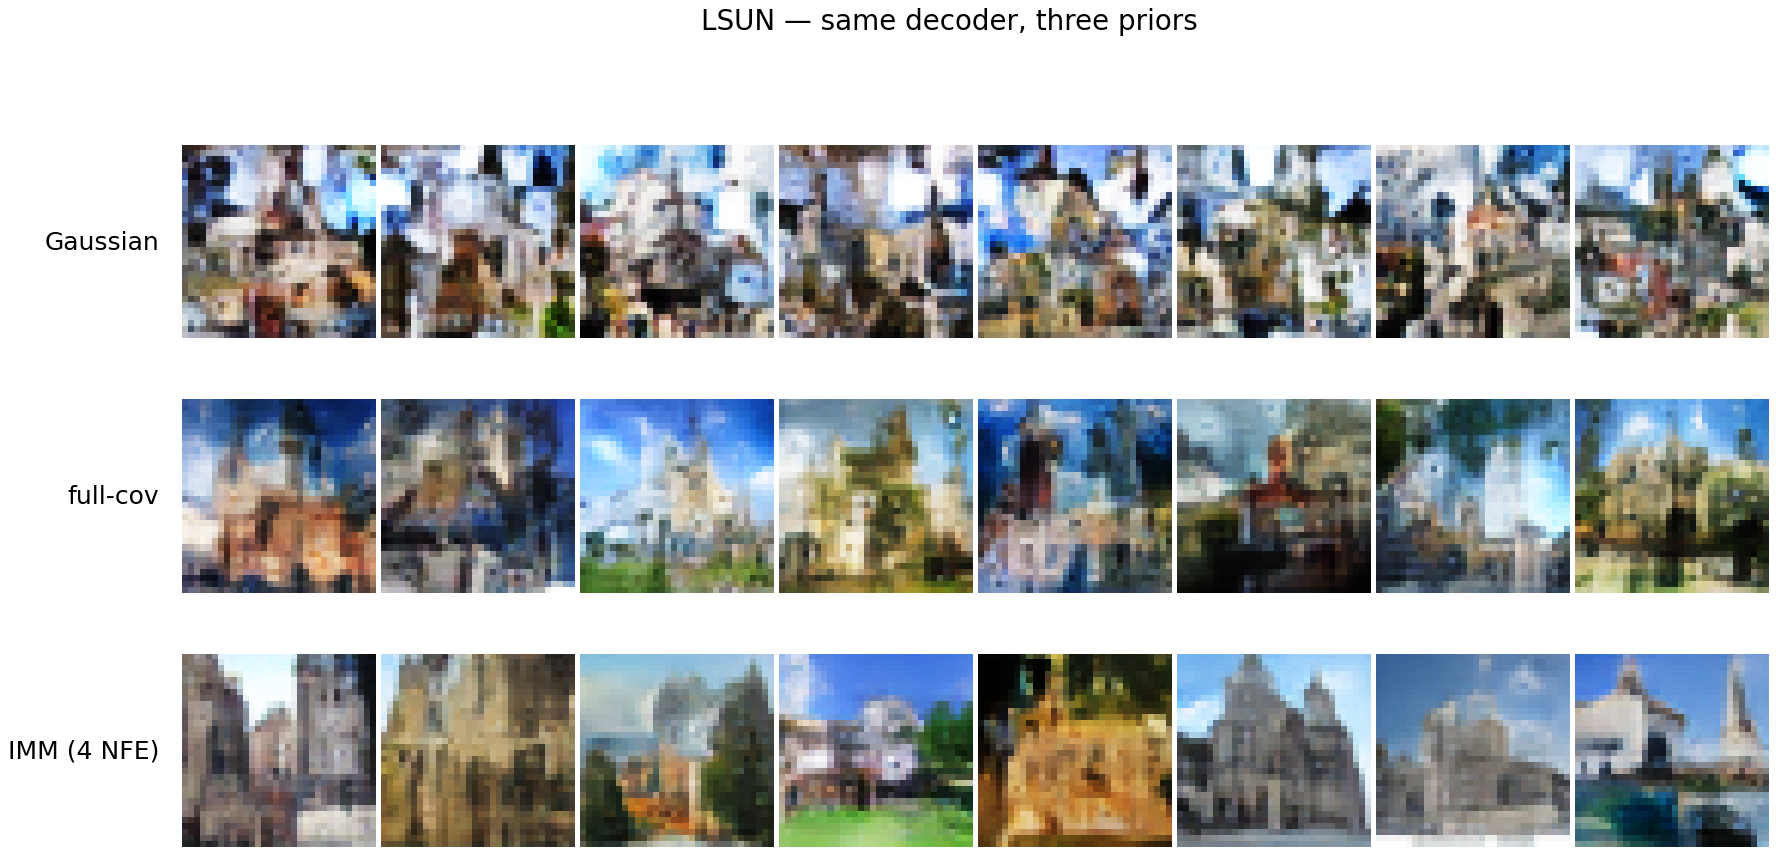
\includegraphics[width=\columnwidth]{figures/compare_LSUN.png}
\caption{LSUN church $32{\times}32$, the only non-face, non-object domain in
the study. Rows as in Figure~\ref{fig:compare}: per-dim Gaussian (FID $152.6$),
full-covariance (FID $79.0$), learned prior at 4 NFE (FID $22.8$).}
\label{fig:lsun}
\end{figure}

\appendix

\section{The VQ rung: codebook collapse and its repair}
\label{app:vq}

Our first VQ autoencoder used loss-based codebook updates and ended with $194$
of $1024$ codes alive after 25 epochs, gaining roughly seven codes per epoch. We
replaced the codebook update with an exponential moving average
(van~den~Oord~et~al., appendix A.1) and ablated the three usual companions.

\begin{table}[h]
\caption{Codebook occupancy after six epochs. EMA alone accounts for the entire
recovery; L2/cosine lookup, dead-code restarts and $k$-means initialization add
nothing measurable on top of it.}
\label{tab:vqabl}
\small
\begin{tabular}{lr}
\toprule
Codebook update & Codes alive \\
\midrule
Loss-based (original), 25 epochs        & 194 / 1024 \\
EMA + L2 + restart + $k$-means          & 1019 / 1024 \\
EMA + restart + $k$-means (no L2)       & 1012 / 1024 \\
EMA only                                & \best{1017 / 1024} \\
\bottomrule
\end{tabular}
\end{table}

The repair improves the compressor and the generator together:

\begin{table}[h]
\caption{Codebook repair, with all generation numbers at $10$k samples for
comparability. The EMA codebook is better on every axis.}
\small
\begin{tabular}{lrr}
\toprule
 & Collapsed & EMA-fixed \\
\midrule
Codes alive                    & 194    & \best{1021} \\
Ceiling (rFID)                 & 5.60   & \best{4.49} \\
Independent marginal codes     & \best{122.84} & 244.84 \\
Autoregressive transformer     & 236.03 & \best{7.33} \\
\bottomrule
\end{tabular}
\end{table}

\paragraph{A sampler bug nearly inverted this conclusion.}
An earlier version of these numbers ($96.8$ collapsed, $197.6$ EMA-fixed) came
from an autoregressive sampler with an off-by-one: the network prepends a BOS
token and drops the last input, so output position $j$ carries
$p(z_j \mid z_{<j})$, and after generating $k$ tokens the sampler read position
$k-1$ instead of $k$. Every token was therefore drawn from the preceding
position's distribution. The symptom was a contradiction rather than a crash:
the code NLL improved $2.6\times$ (from $5.34$ to $2.03$) while FID moved by
$5\%$. A model that predicts that well cannot sample that badly. With the
sampler corrected --- verified by training on a single fixed sequence and
recovering it exactly --- the same checkpoints give $236.03$ and $7.33$.

We report the episode because the erroneous numbers were self-consistent and
supported a plausible story (that fixing collapse shifts difficulty onto the
prior). Only the likelihood/FID mismatch flagged it. Where a generative model is
evaluated by sample quality alone, a bug in the sampler is invisible; the
likelihood is what made it detectable.

At $50$k samples the corrected pipeline reaches FID $6.571$ against a ceiling of
$3.48$, i.e.\ it closes $98.7\%$ of the distance from its free baseline to its
ceiling --- the same as the adversarial autoencoder on that measure ($98.2\%$),
at essentially the same FID ($6.29$). Truncation hurts: $T{=}1.0$ without top-$k$ is
best, and top-$k{=}100$ costs $6.6$ FID.

\section{Reconstruction and timing}
\label{app:support}

Table~\ref{tab:recon} reports conventional reconstruction metrics for the
capacity-matched compressors of Table~\ref{tab:diagnostic} and for the
over-complete NVAE, and Table~\ref{tab:time} puts the
efficiency claim on a clock. Neither carries an argument in the main text; both
are here so the numbers behind Sections~\ref{sec:nogap} and~\ref{sec:results}
are available.

\begin{table}[t]
\caption{Reconstruction on $10$k held-out CelebA images. All compressors use a
$256$-dimensional latent except the over-complete NVAE rows, which use
$21{,}504$. ``bpd'' is a discretised-Gaussian NLL bound, not an exact bits/dim,
and includes the KL only for the NVAE rows where an ELBO exists. Among
matched-capacity models the ordering follows the training objective: the
$\sigma$-VAE leads on PSNR/SSIM, the adversarial autoencoder on LPIPS --- which
is what its loss optimises --- and quantisation costs VQ about $3$\,dB.}
\label{tab:recon}
\small
\begin{tabular}{lrrrr}
\toprule
Compressor & PSNR $\uparrow$ & SSIM $\uparrow$ & LPIPS $\downarrow$ & bpd $\downarrow$ \\
\midrule
Adversarial AE            & 30.45 & 0.9425 & \best{0.0027} & 5.085 \\
$\sigma$-VAE              & \best{31.38} & \best{0.9498} & 0.0050 & 4.919 \\
VQ-VAE (256 codes)        & 26.98 & 0.8992 & 0.0063 & 5.646 \\
VQ-VAE (1024 codes)       & 27.61 & 0.9029 & 0.0054 & 5.537 \\
NVAE matched              & 29.95 & 0.9333 & 0.0089 & 5.398 \\
NVAE matched + sched.\ samp.\ & 29.28 & 0.9236 & 0.0121 & 5.475 \\
\midrule
\multicolumn{5}{l}{\emph{$7\times$ over-complete, not capacity-matched}}\\
NVAE over-complete (BN)   & 44.05 & 0.9955 & 0.0001 & 4.053 \\
NVAE over-complete (GN)   & 45.14 & 0.9965 & 0.0001 & 4.036 \\
\bottomrule
\end{tabular}
\end{table}

\begin{table}[t]
\caption{Wall-clock sampling cost, milliseconds per $1000$ images (RTX~5070~Ti,
batch $250$, CUDA-synchronised, 4 repeats). NFE alone is not an efficiency
measure: the latent DDPM is a 6-block MLP over a $64$-d vector while the conv
priors are $4.64$M-parameter CNNs over a latent grid, so a step is not a step.
Decode costs differ between stacks and totals should be compared within a
stack.}
\label{tab:time}
\small
\begin{tabular}{llrrr}
\toprule
Stack & Prior & NFE & Sample & Total \\
\midrule
\multicolumn{5}{l}{\emph{Perceptual--adversarial AE} (decode $65.4$)}\\
& full-cov Gaussian & 0  & 0.4   & 65.8 \\
& IMM conv          & 1  & 26.6  & 92.0 \\
& IMM conv          & 2  & 55.2  & 120.6 \\
& IMM conv          & 4  & 109.2 & \best{174.6} \\
& IMM conv          & 16 & 445.5 & 510.8 \\
\midrule
\multicolumn{5}{l}{\emph{MSE NVAE} (decode $10.6$)}\\
& IMM-legacy (MLP)  & 16   & 98.9   & 109.6 \\
& latent DDPM (MLP) & 100  & 681.7  & 692.3 \\
& latent DDPM (MLP) & 1000 & 6053.1 & 6063.7 \\
\bottomrule
\end{tabular}
\end{table}

\section{Sample grids}
\label{app:grids}

Every figure uses 8 columns at $4\times$ nearest-neighbour upscaling. Nearest,
not bilinear: these are $32{\times}32$ images and smoothing them would invent
detail the model did not produce, which is the wrong thing to do in a figure
about sample sharpness.

\begin{figure}[h]
\centering
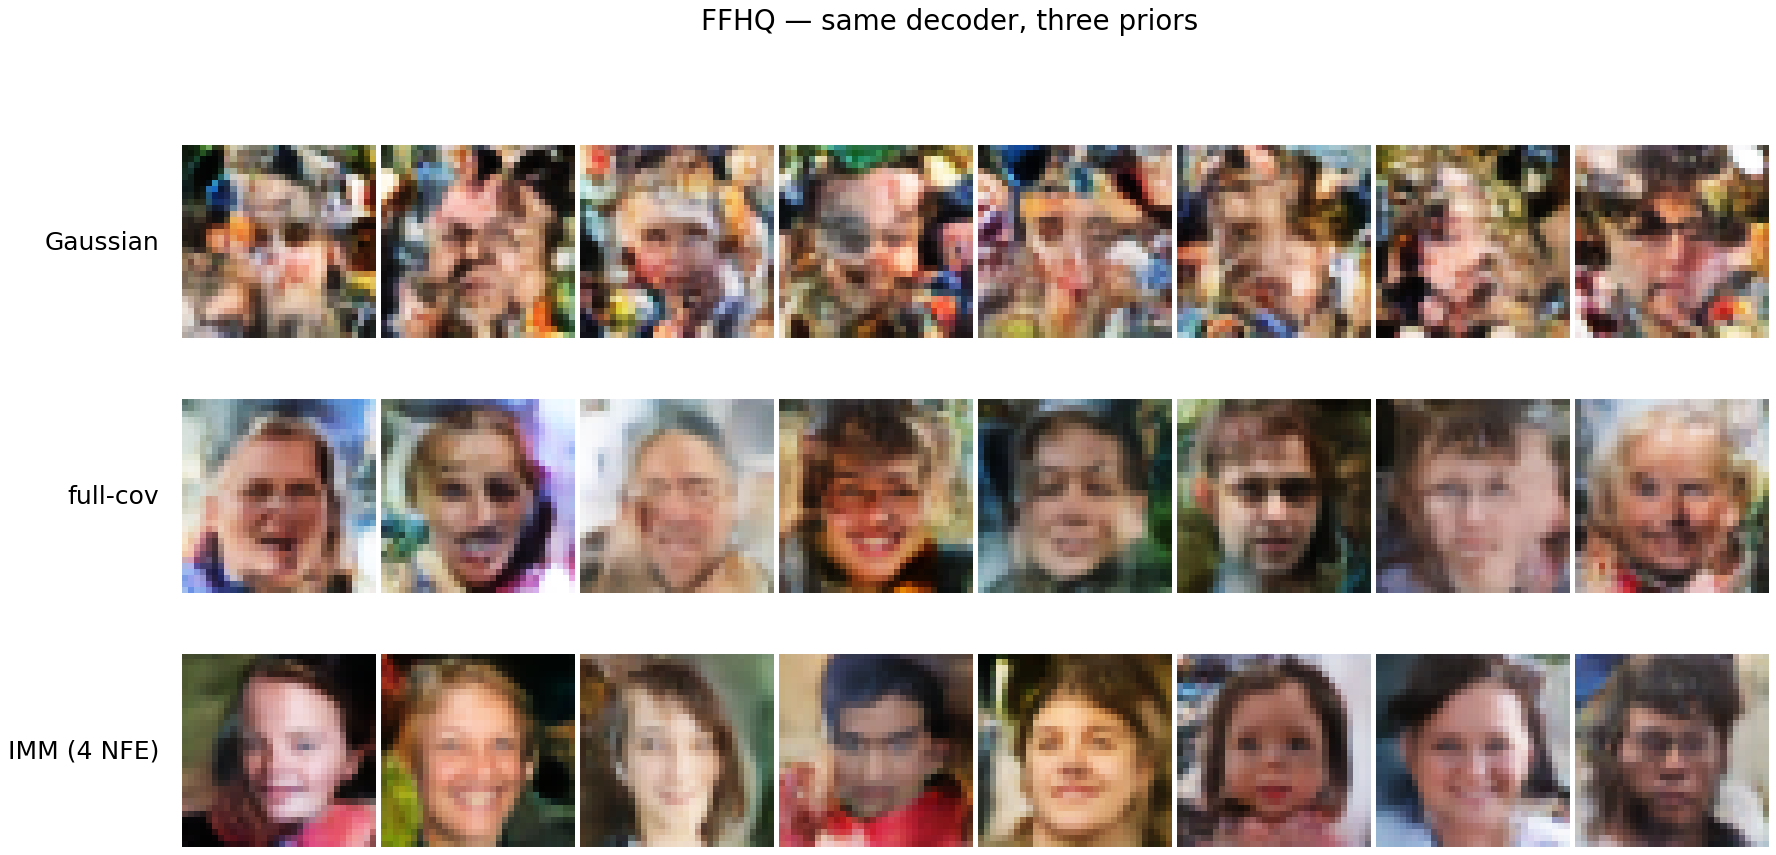
\includegraphics[width=\columnwidth]{figures/compare_FFHQ.png}\\[2pt]
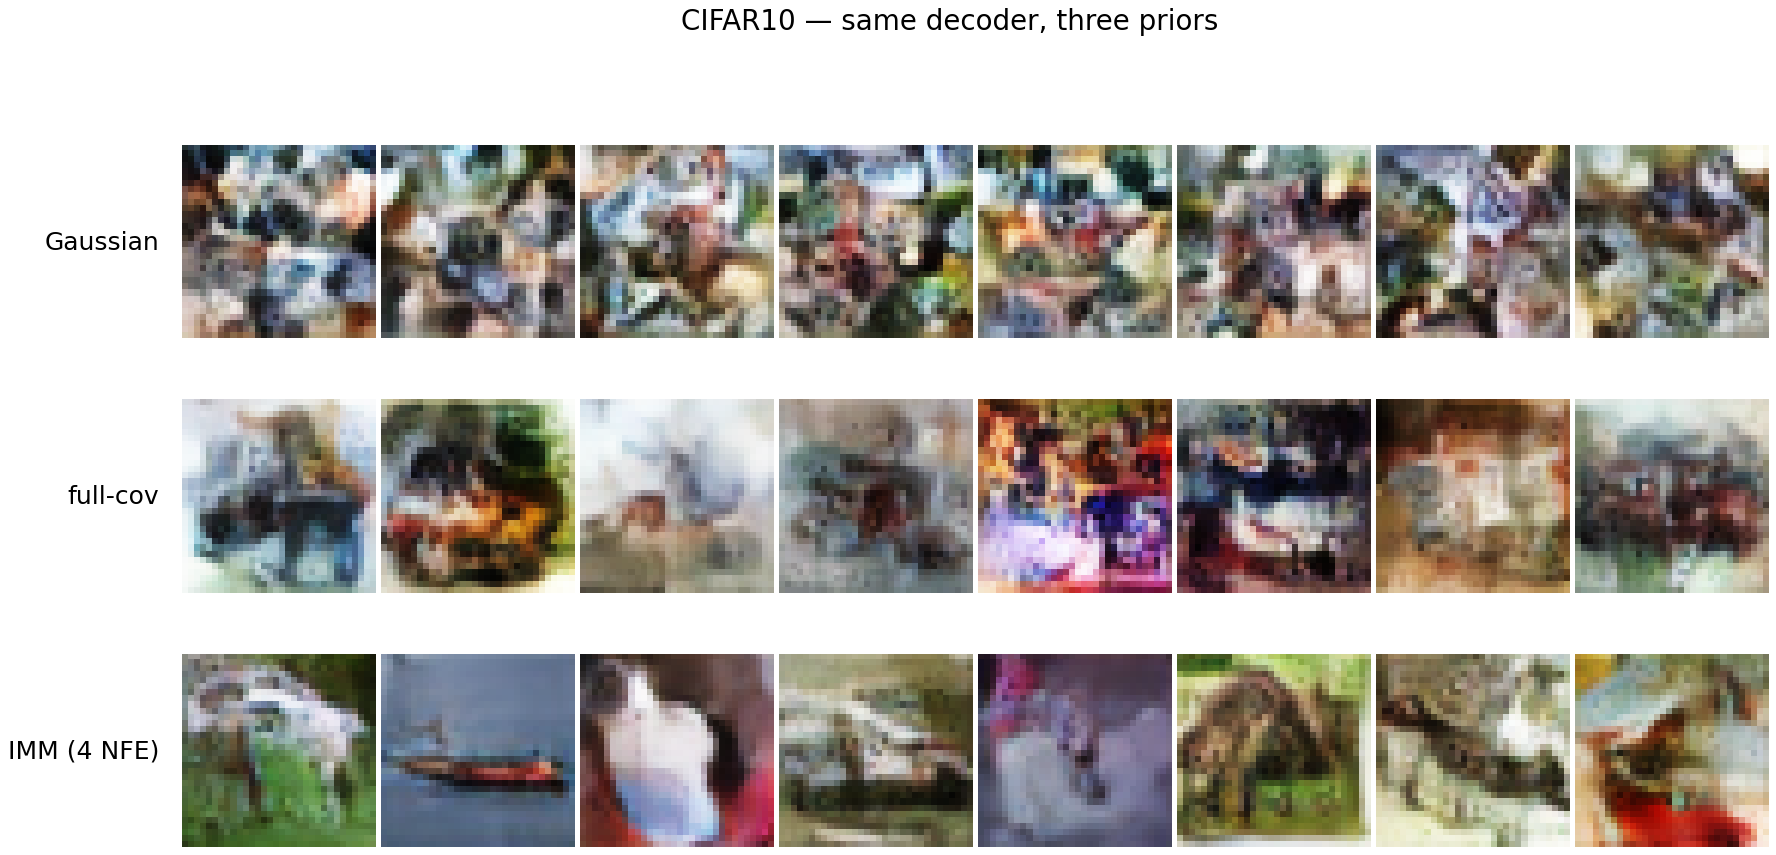
\includegraphics[width=\columnwidth]{figures/compare_CIFAR10.png}\\[2pt]
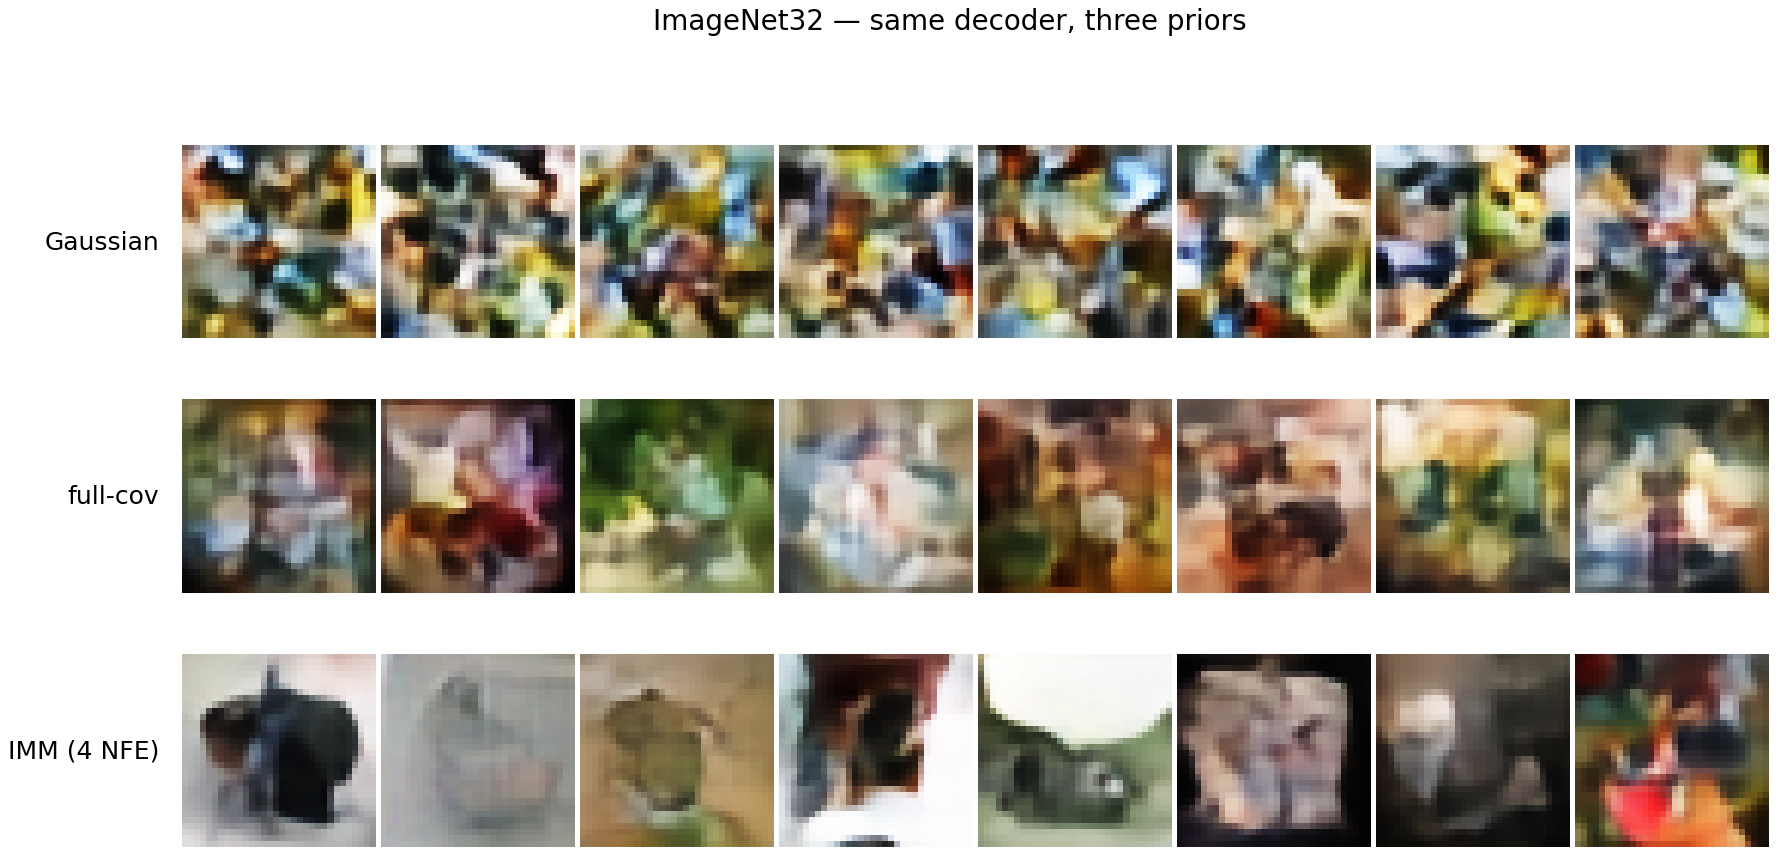
\includegraphics[width=\columnwidth]{figures/compare_ImageNet32.png}\\[2pt]
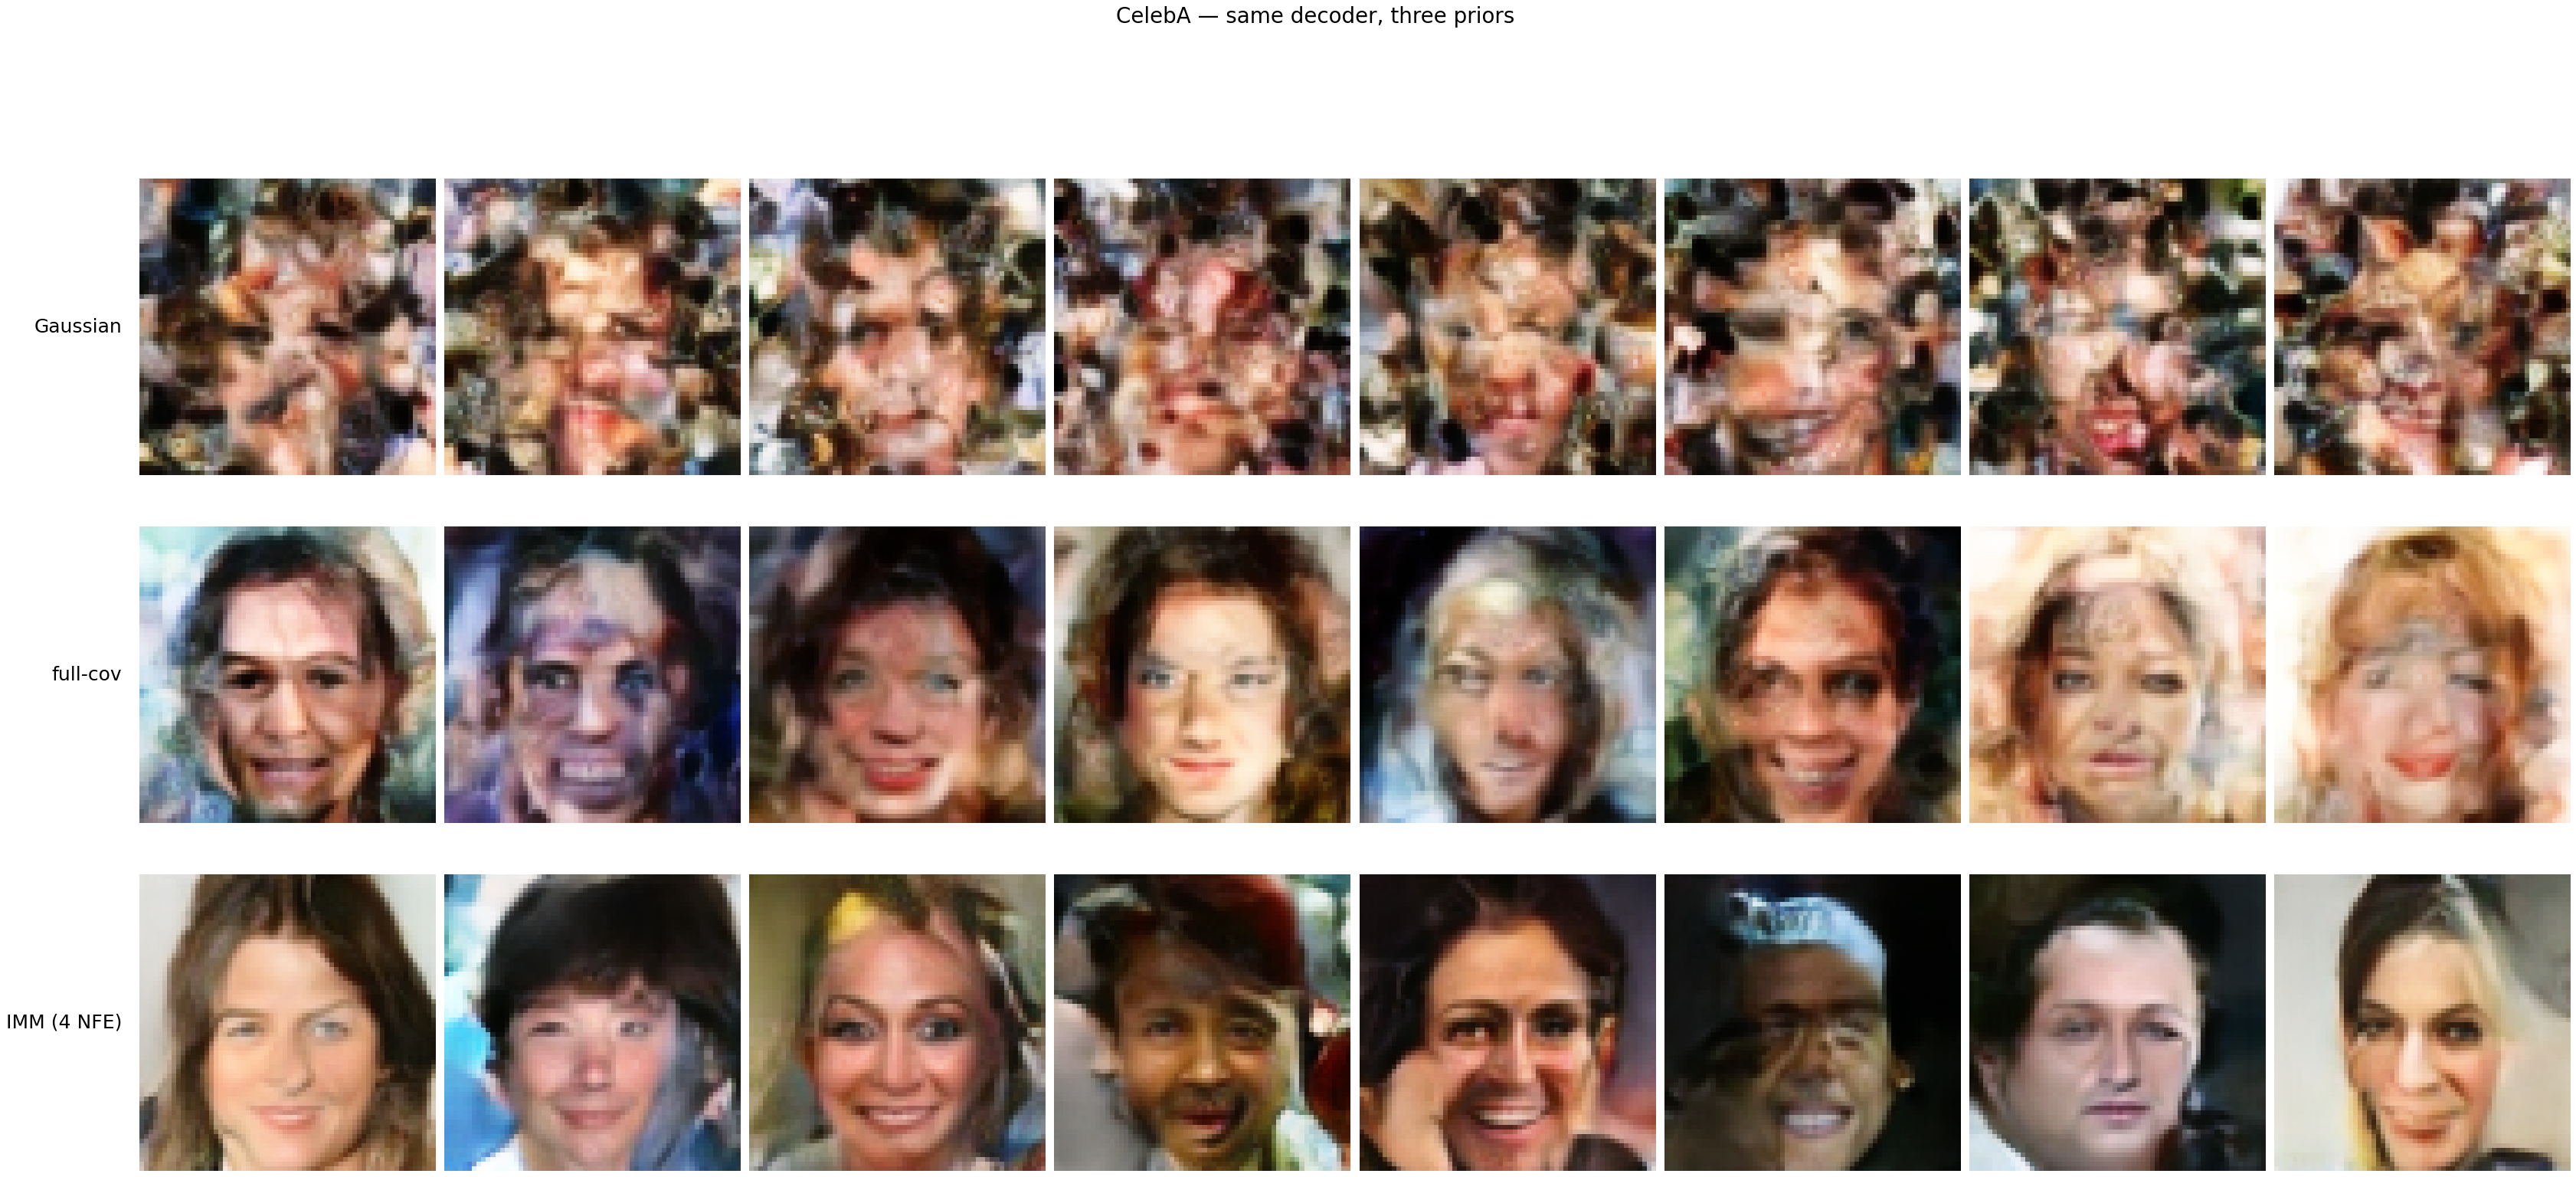
\includegraphics[width=\columnwidth]{figures/compare_CelebA64.png}
\caption{Per-dim Gaussian / full-covariance / learned prior on the remaining
four settings, matching Figure~\ref{fig:compare}. The progression is the same
everywhere, and the covariance control's samples are visibly less varied than
the learned prior's --- the qualitative form of the recall gap in
Table~\ref{tab:prdc}.}
\label{fig:compare-rest}
\end{figure}

\begin{figure}[h]
\centering
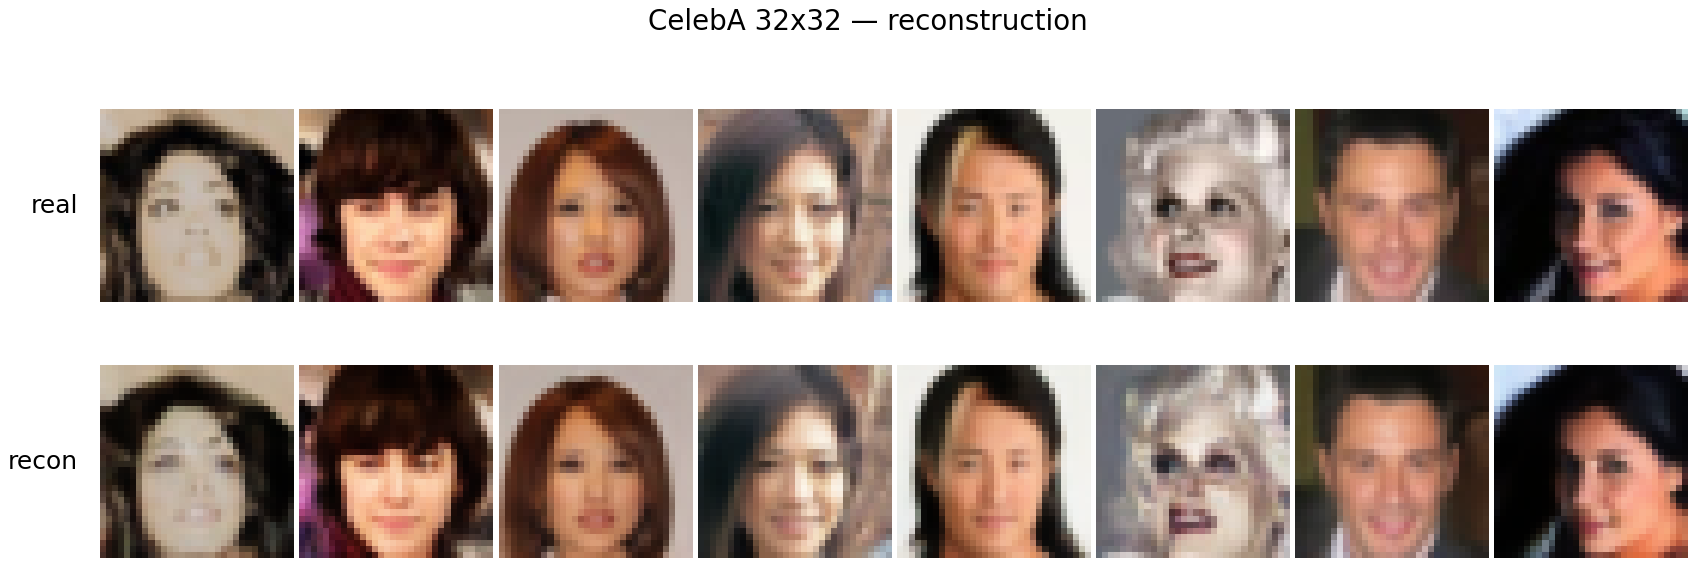
\includegraphics[width=\columnwidth]{figures/reconstructions_CelebA.png}\\[2pt]
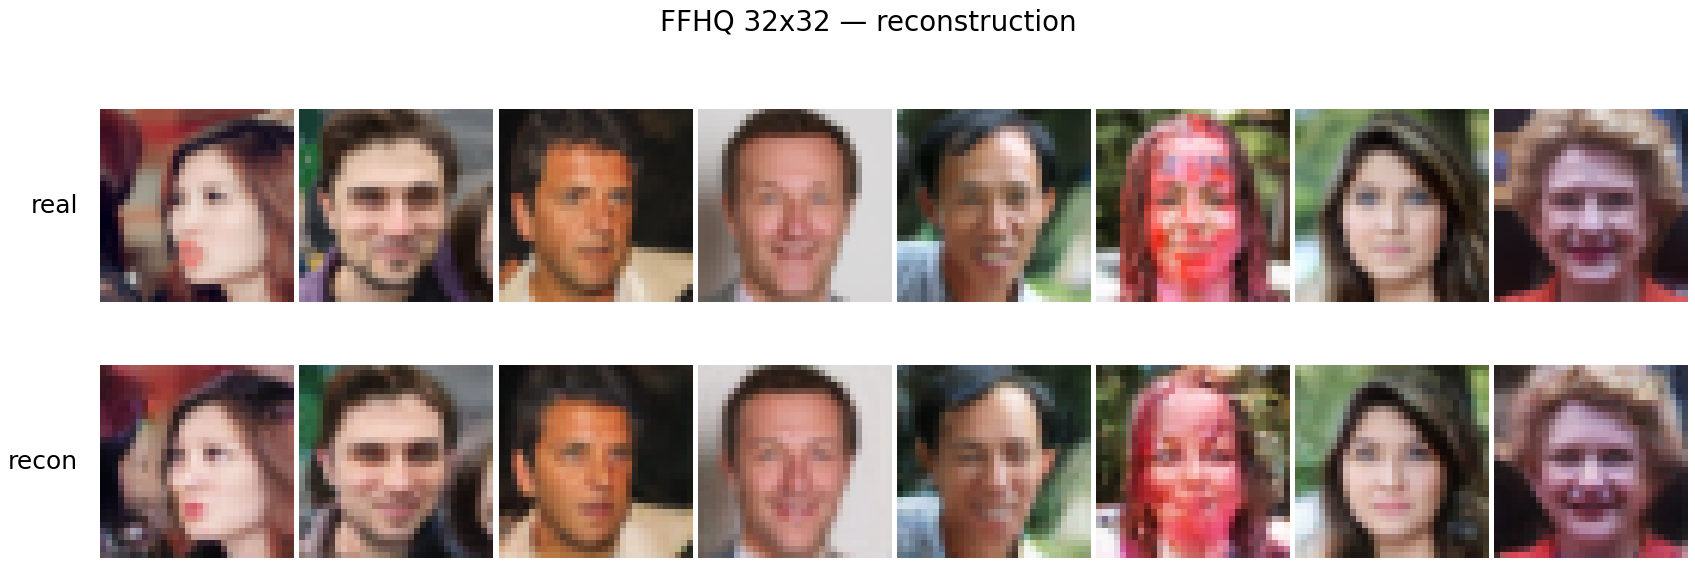
\includegraphics[width=\columnwidth]{figures/reconstructions_FFHQ.png}\\[2pt]
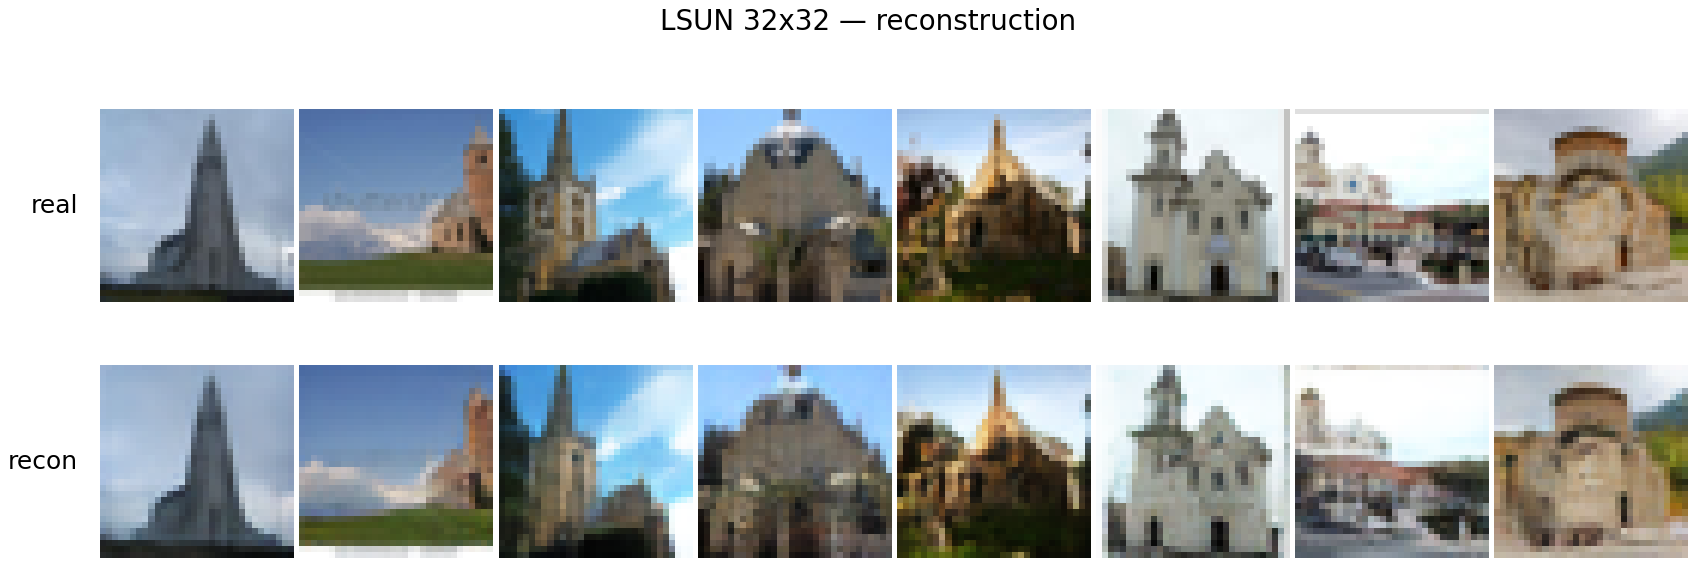
\includegraphics[width=\columnwidth]{figures/reconstructions_LSUN.png}\\[2pt]
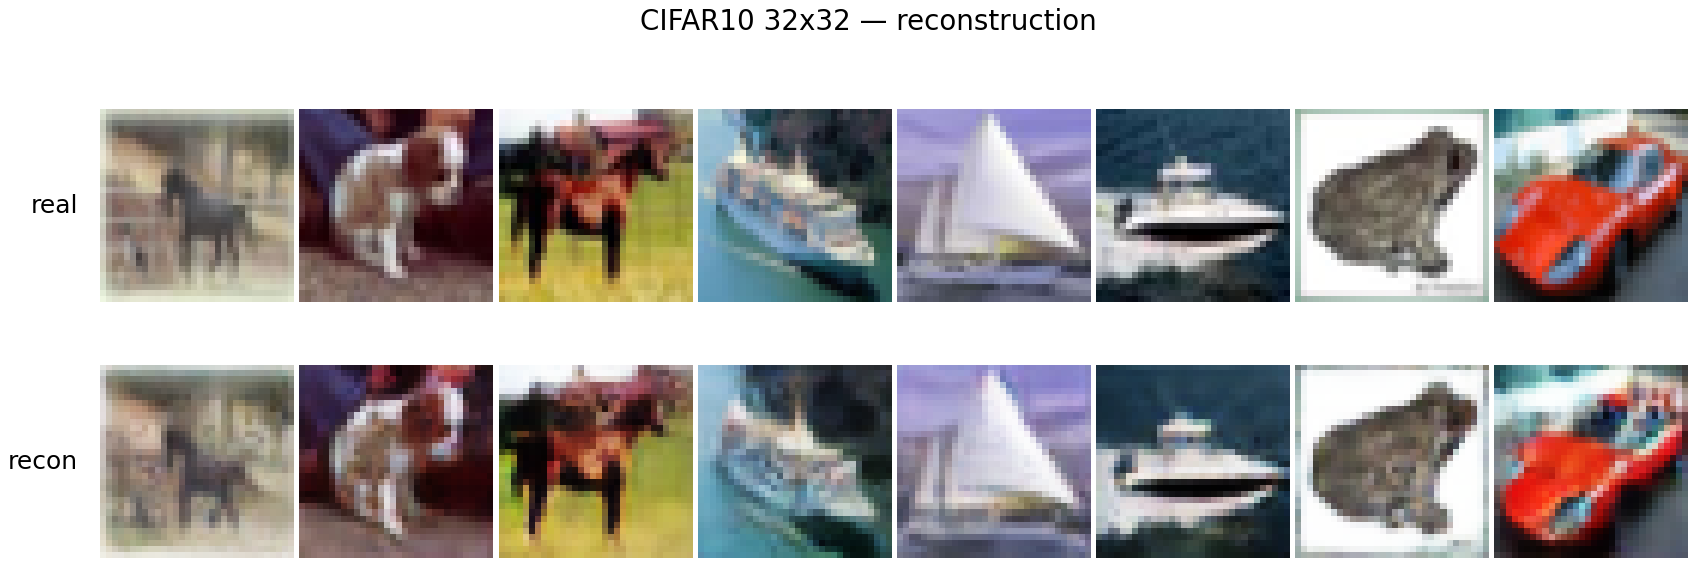
\includegraphics[width=\columnwidth]{figures/reconstructions_CIFAR10.png}\\[2pt]
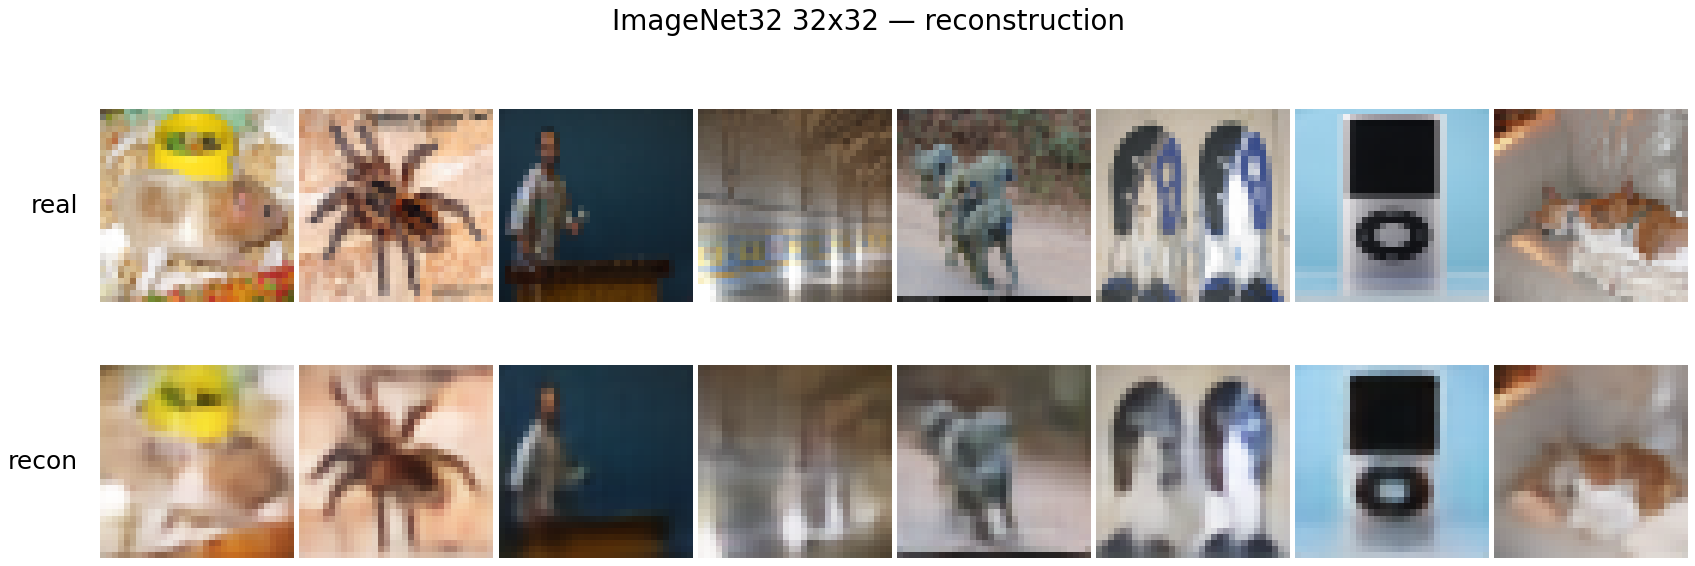
\includegraphics[width=\columnwidth]{figures/reconstructions_ImageNet32.png}\\[2pt]
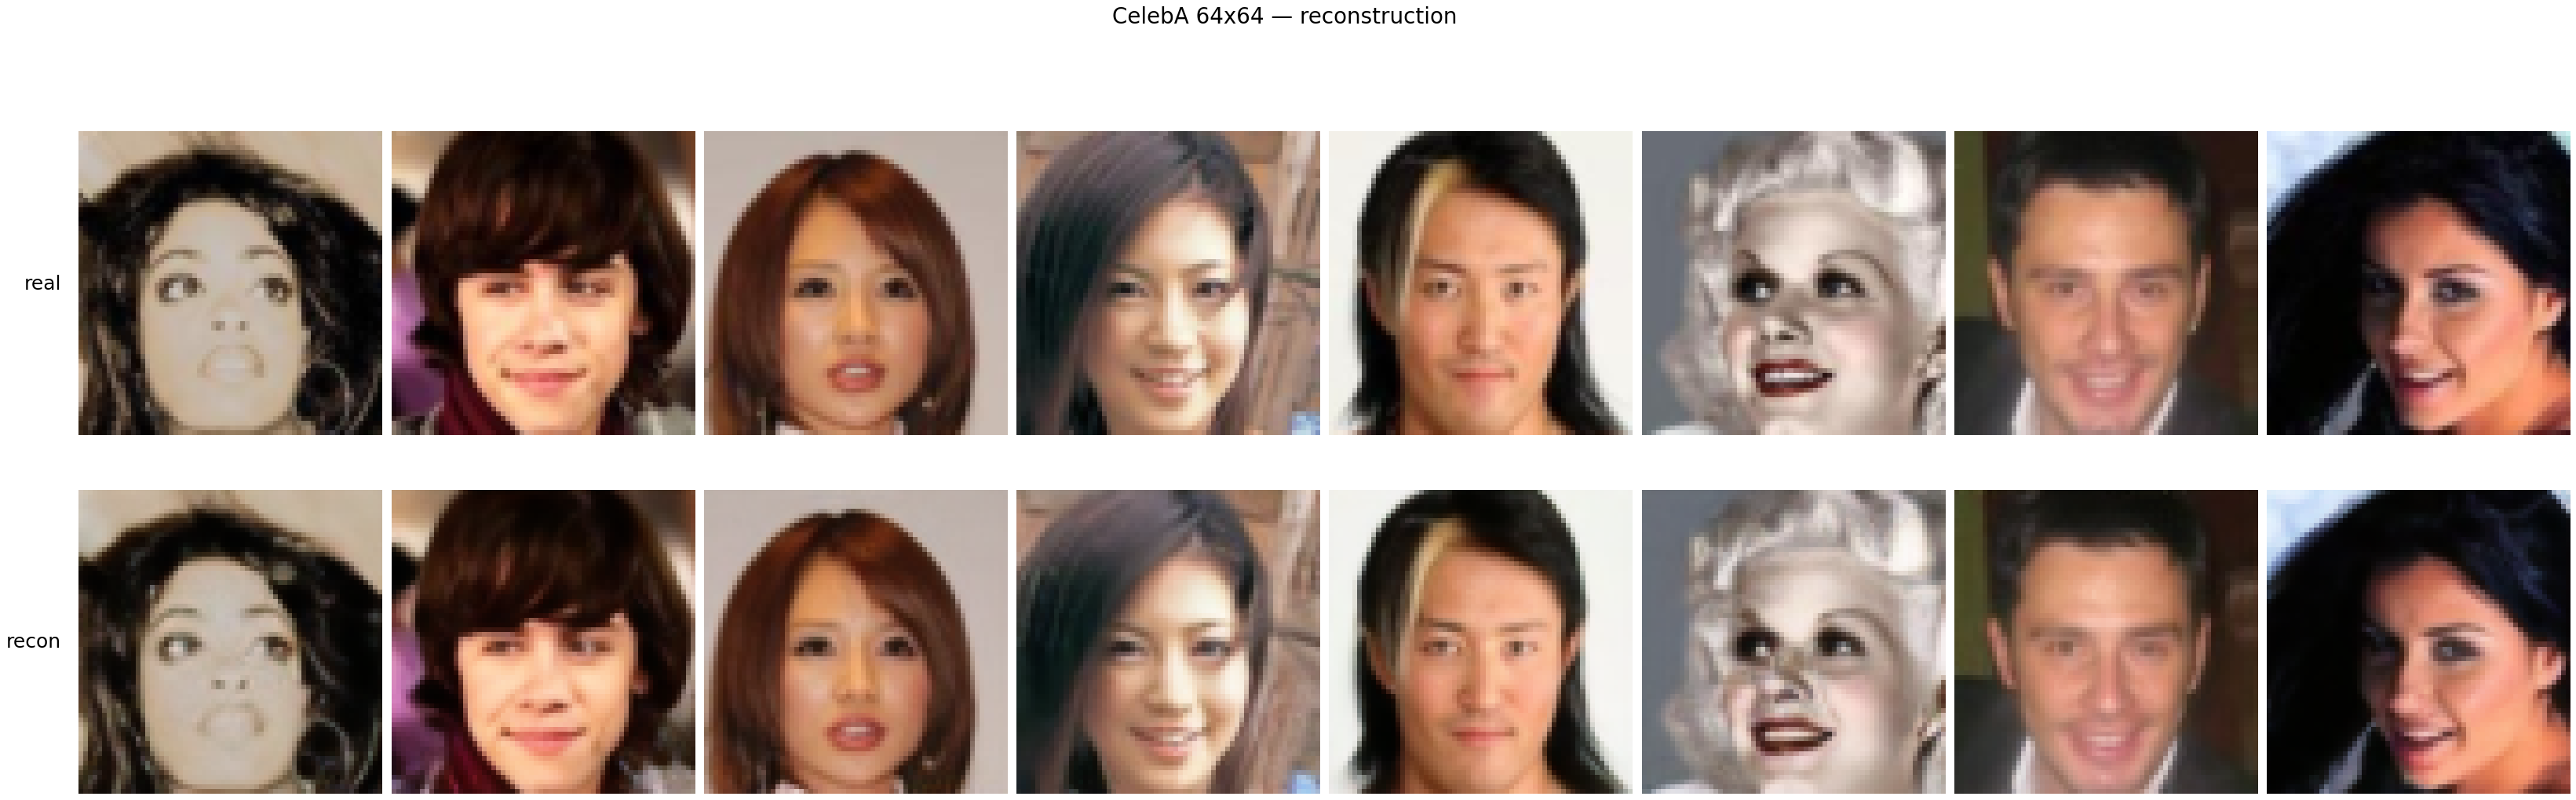
\includegraphics[width=\columnwidth]{figures/reconstructions_CelebA64.png}
\caption{Held-out images (top row of each pair) and their reconstructions. These
are the ceilings of Table~\ref{tab:main}: no prior can produce anything the
decoder cannot already reproduce here.}
\label{fig:recons}
\end{figure}

\begin{figure}[h]
\centering
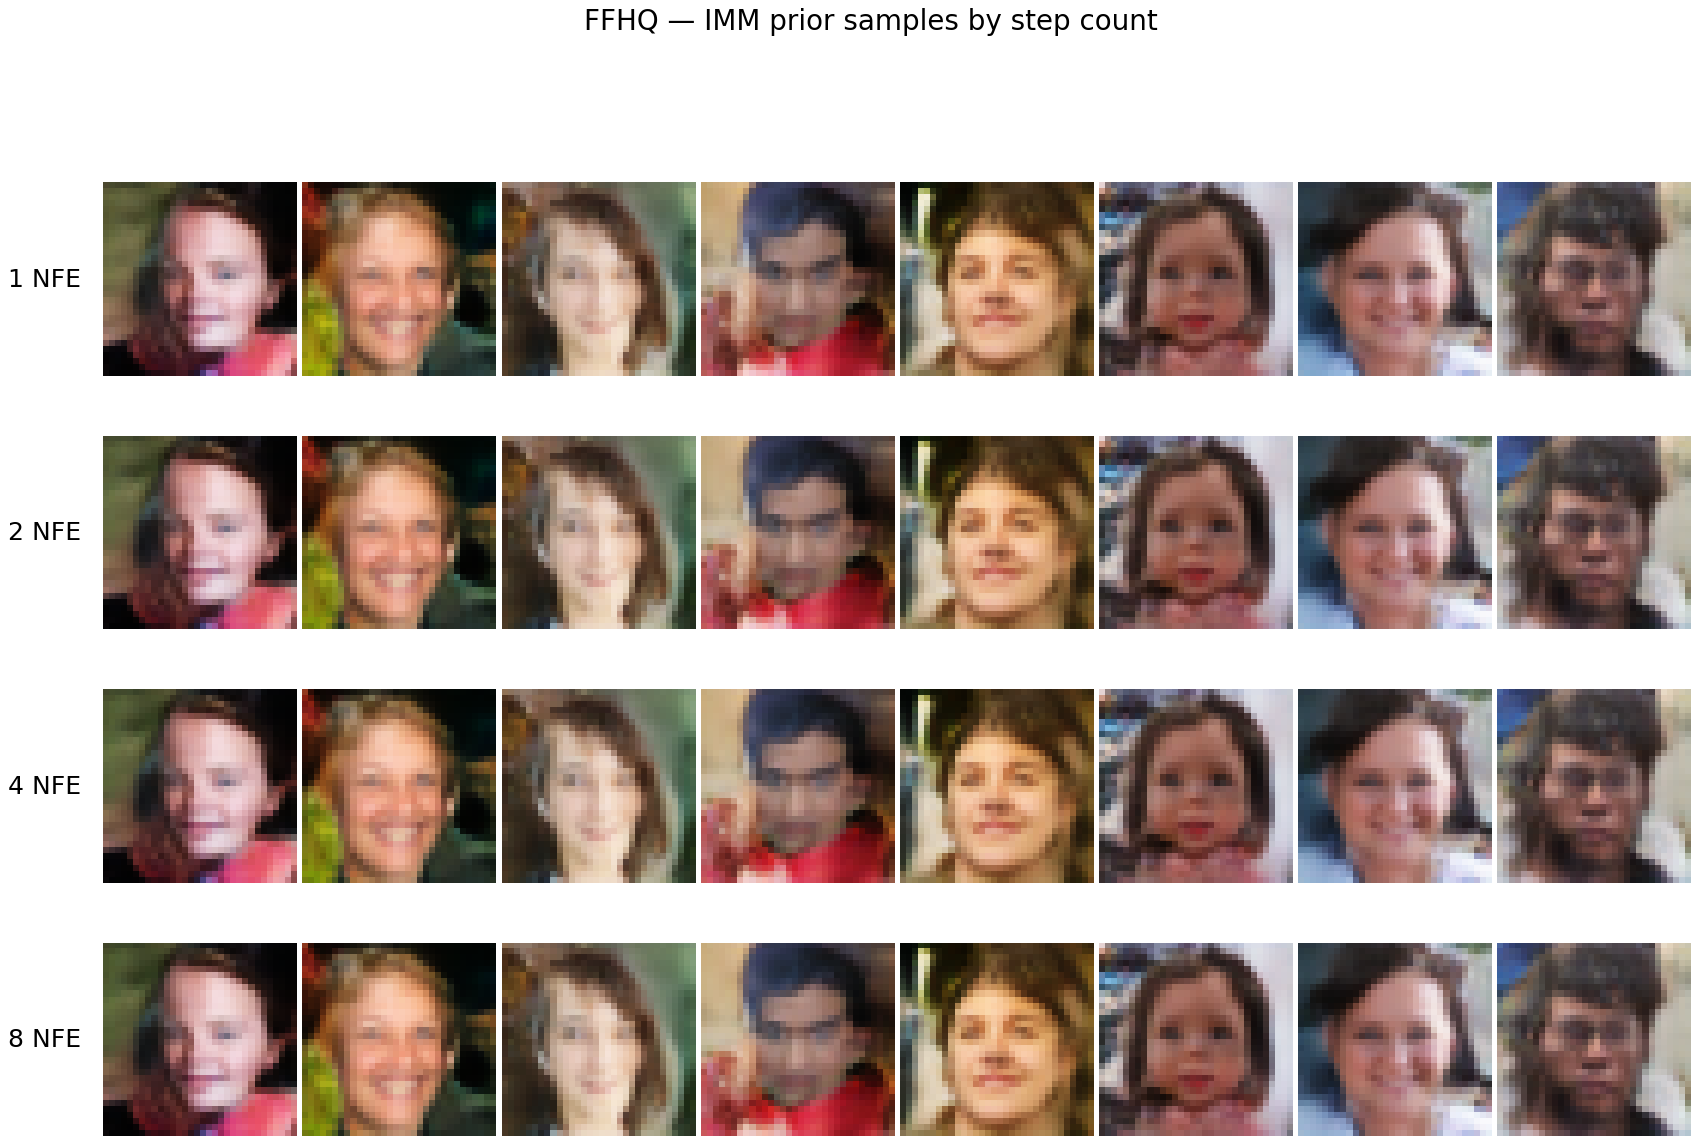
\includegraphics[width=\columnwidth]{figures/samples_FFHQ.png}\\[2pt]
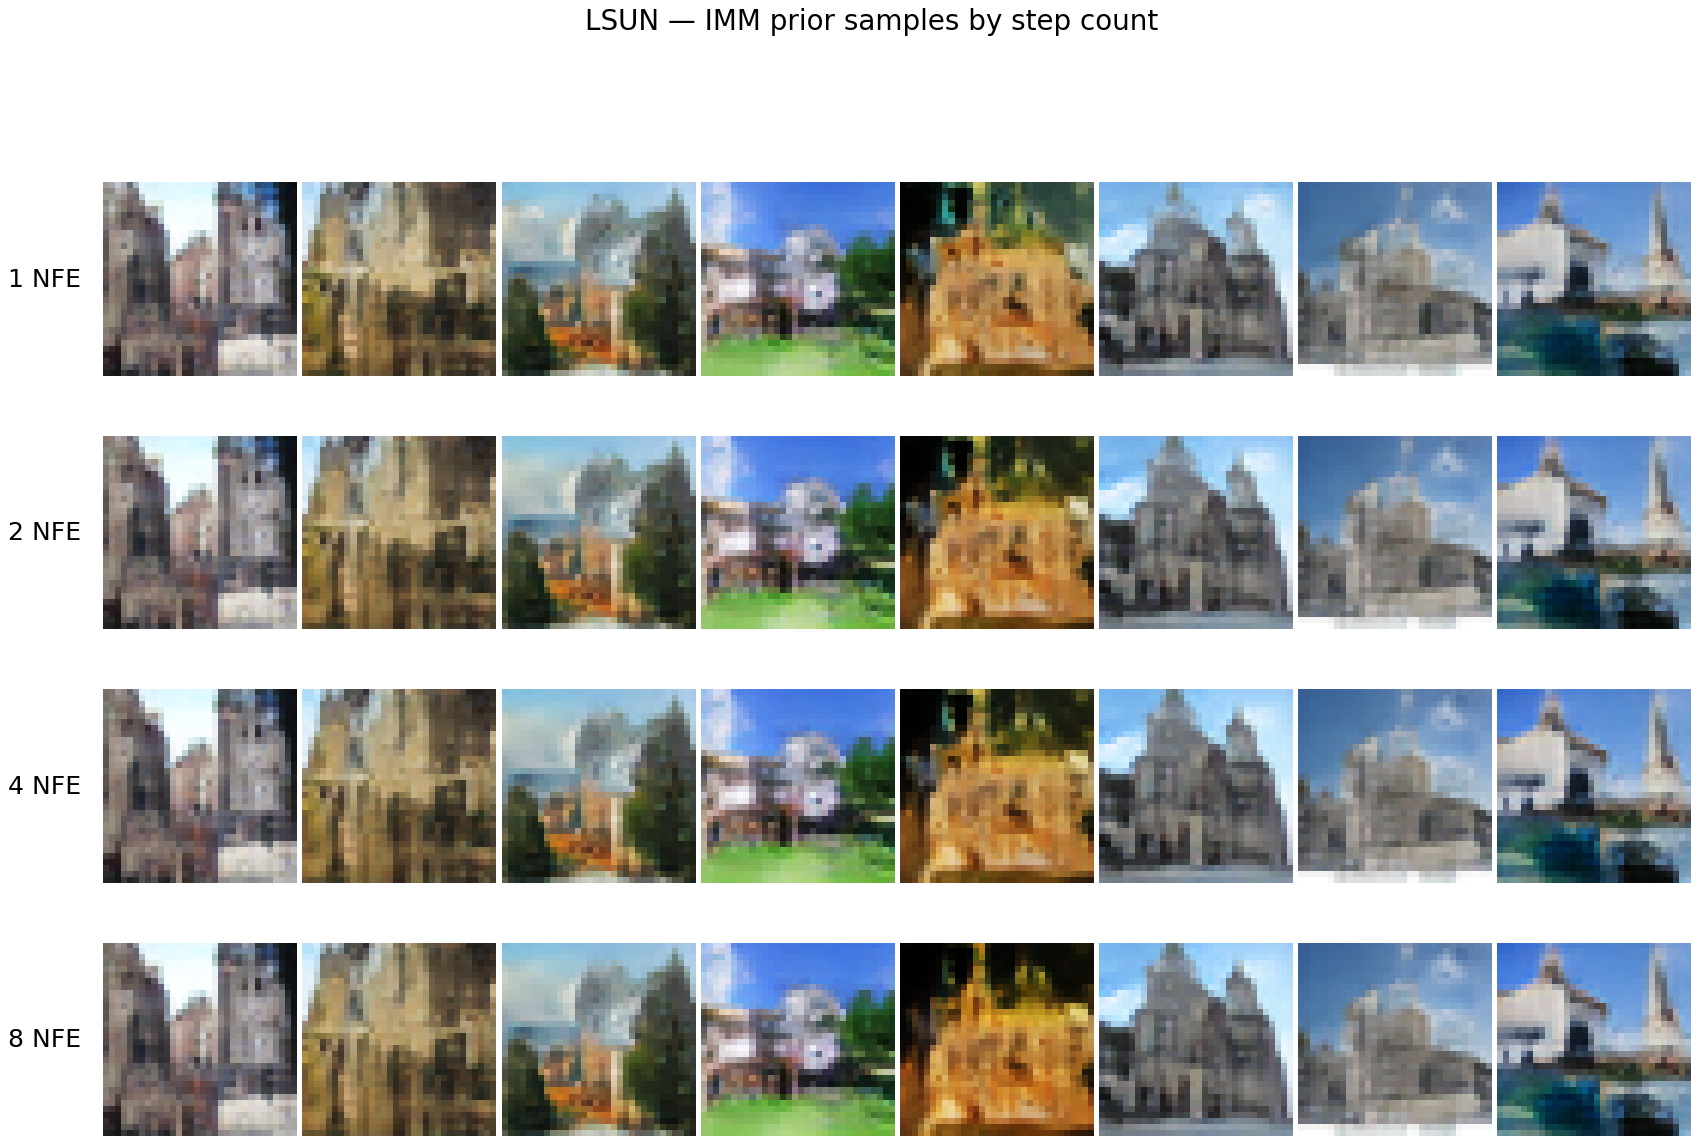
\includegraphics[width=\columnwidth]{figures/samples_LSUN.png}\\[2pt]
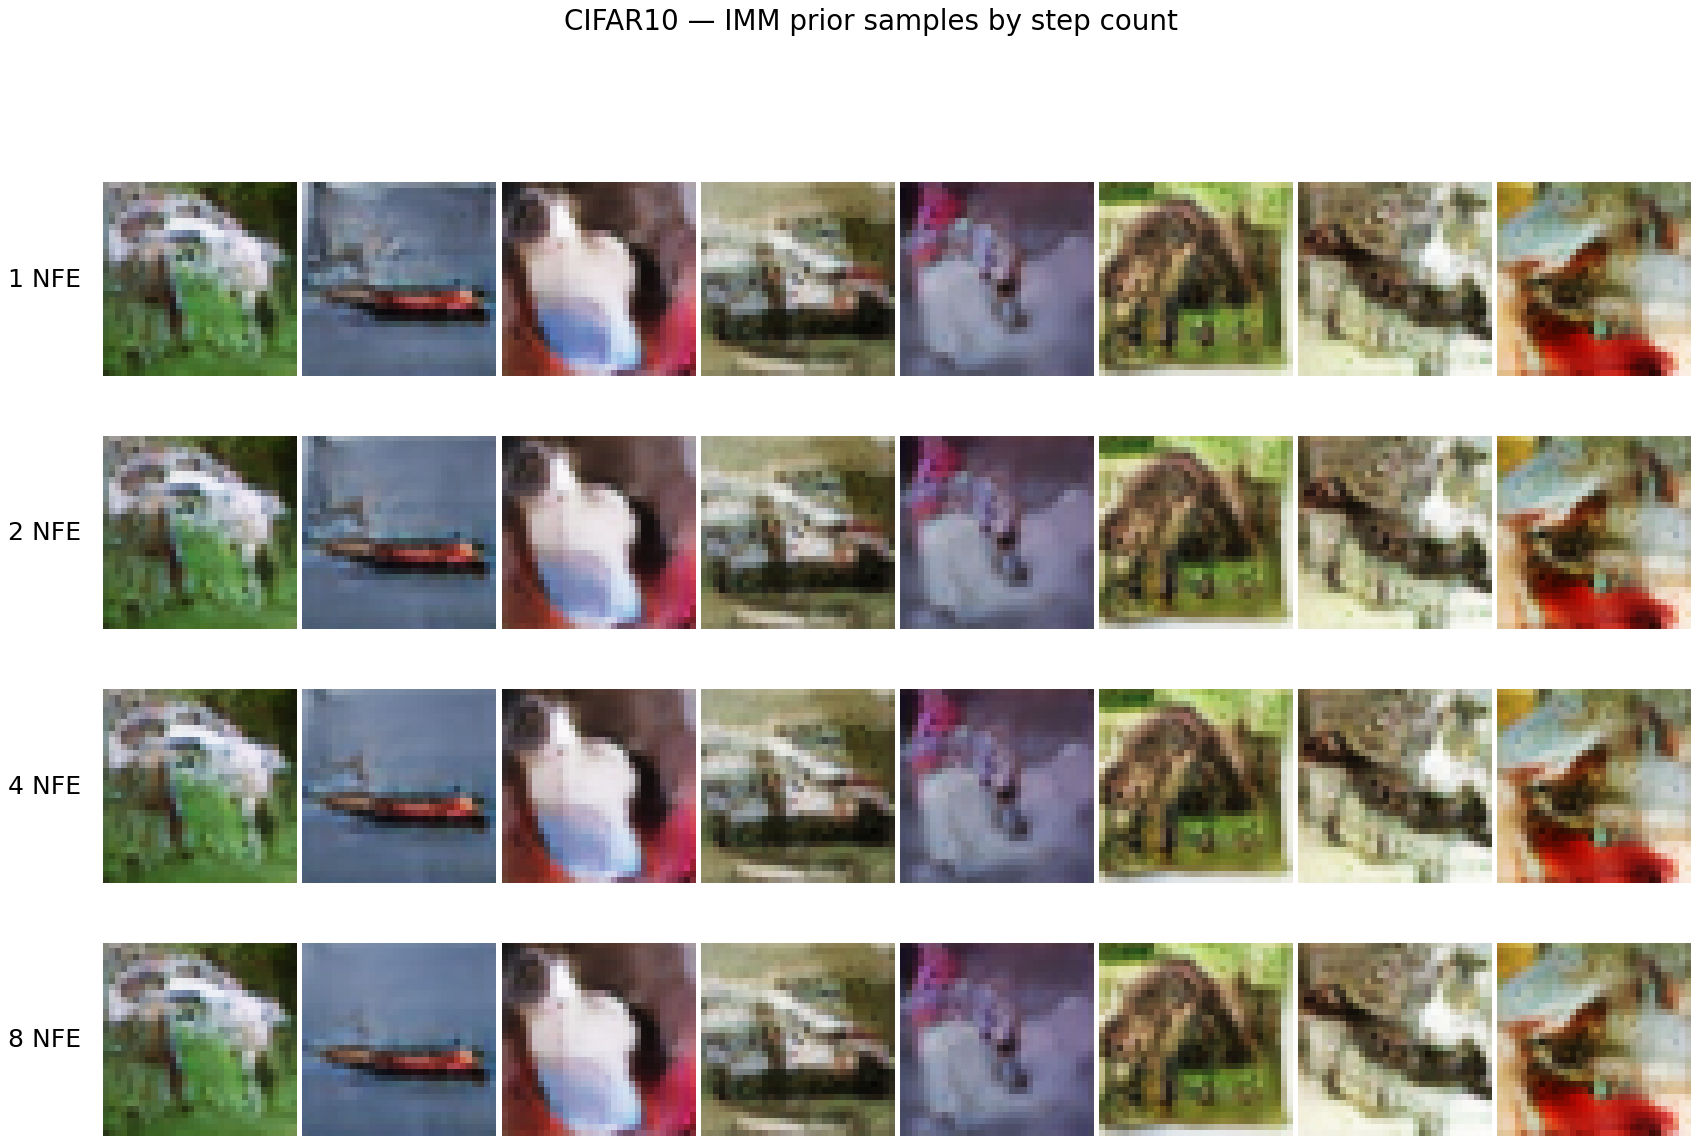
\includegraphics[width=\columnwidth]{figures/samples_CIFAR10.png}\\[2pt]
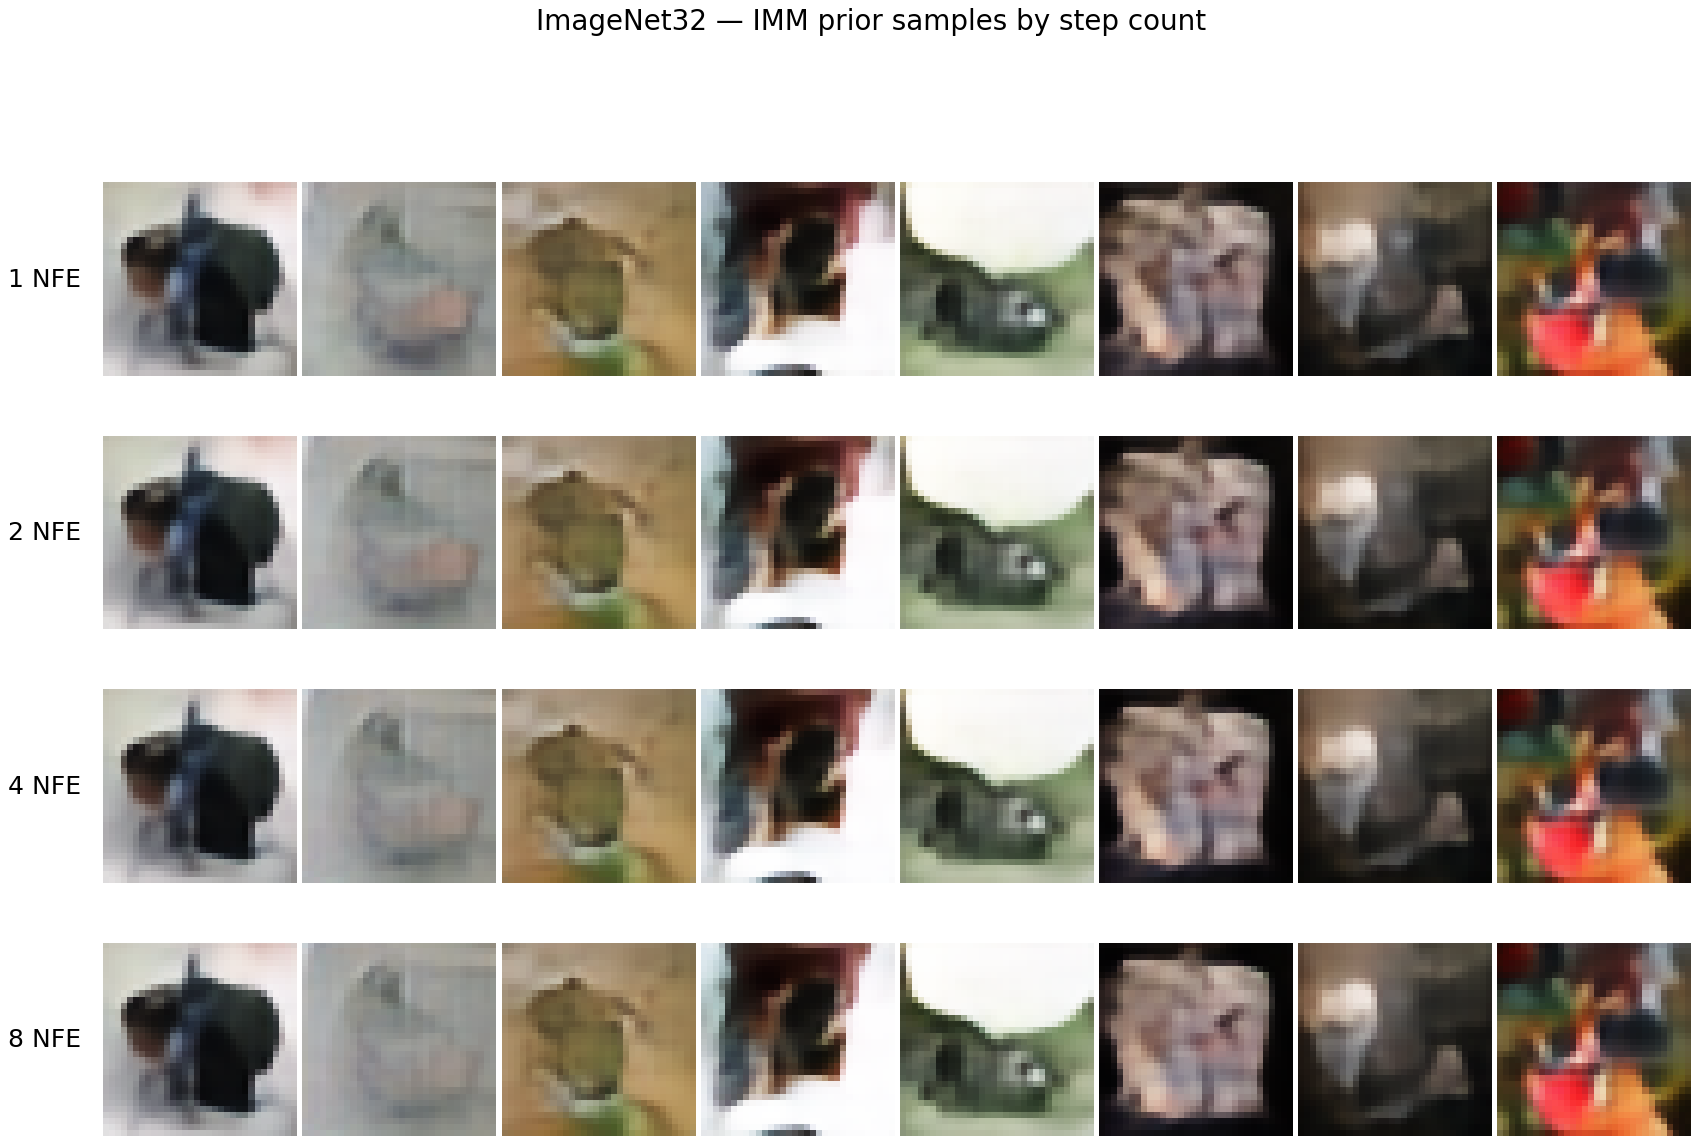
\includegraphics[width=\columnwidth]{figures/samples_ImageNet32.png}\\[2pt]
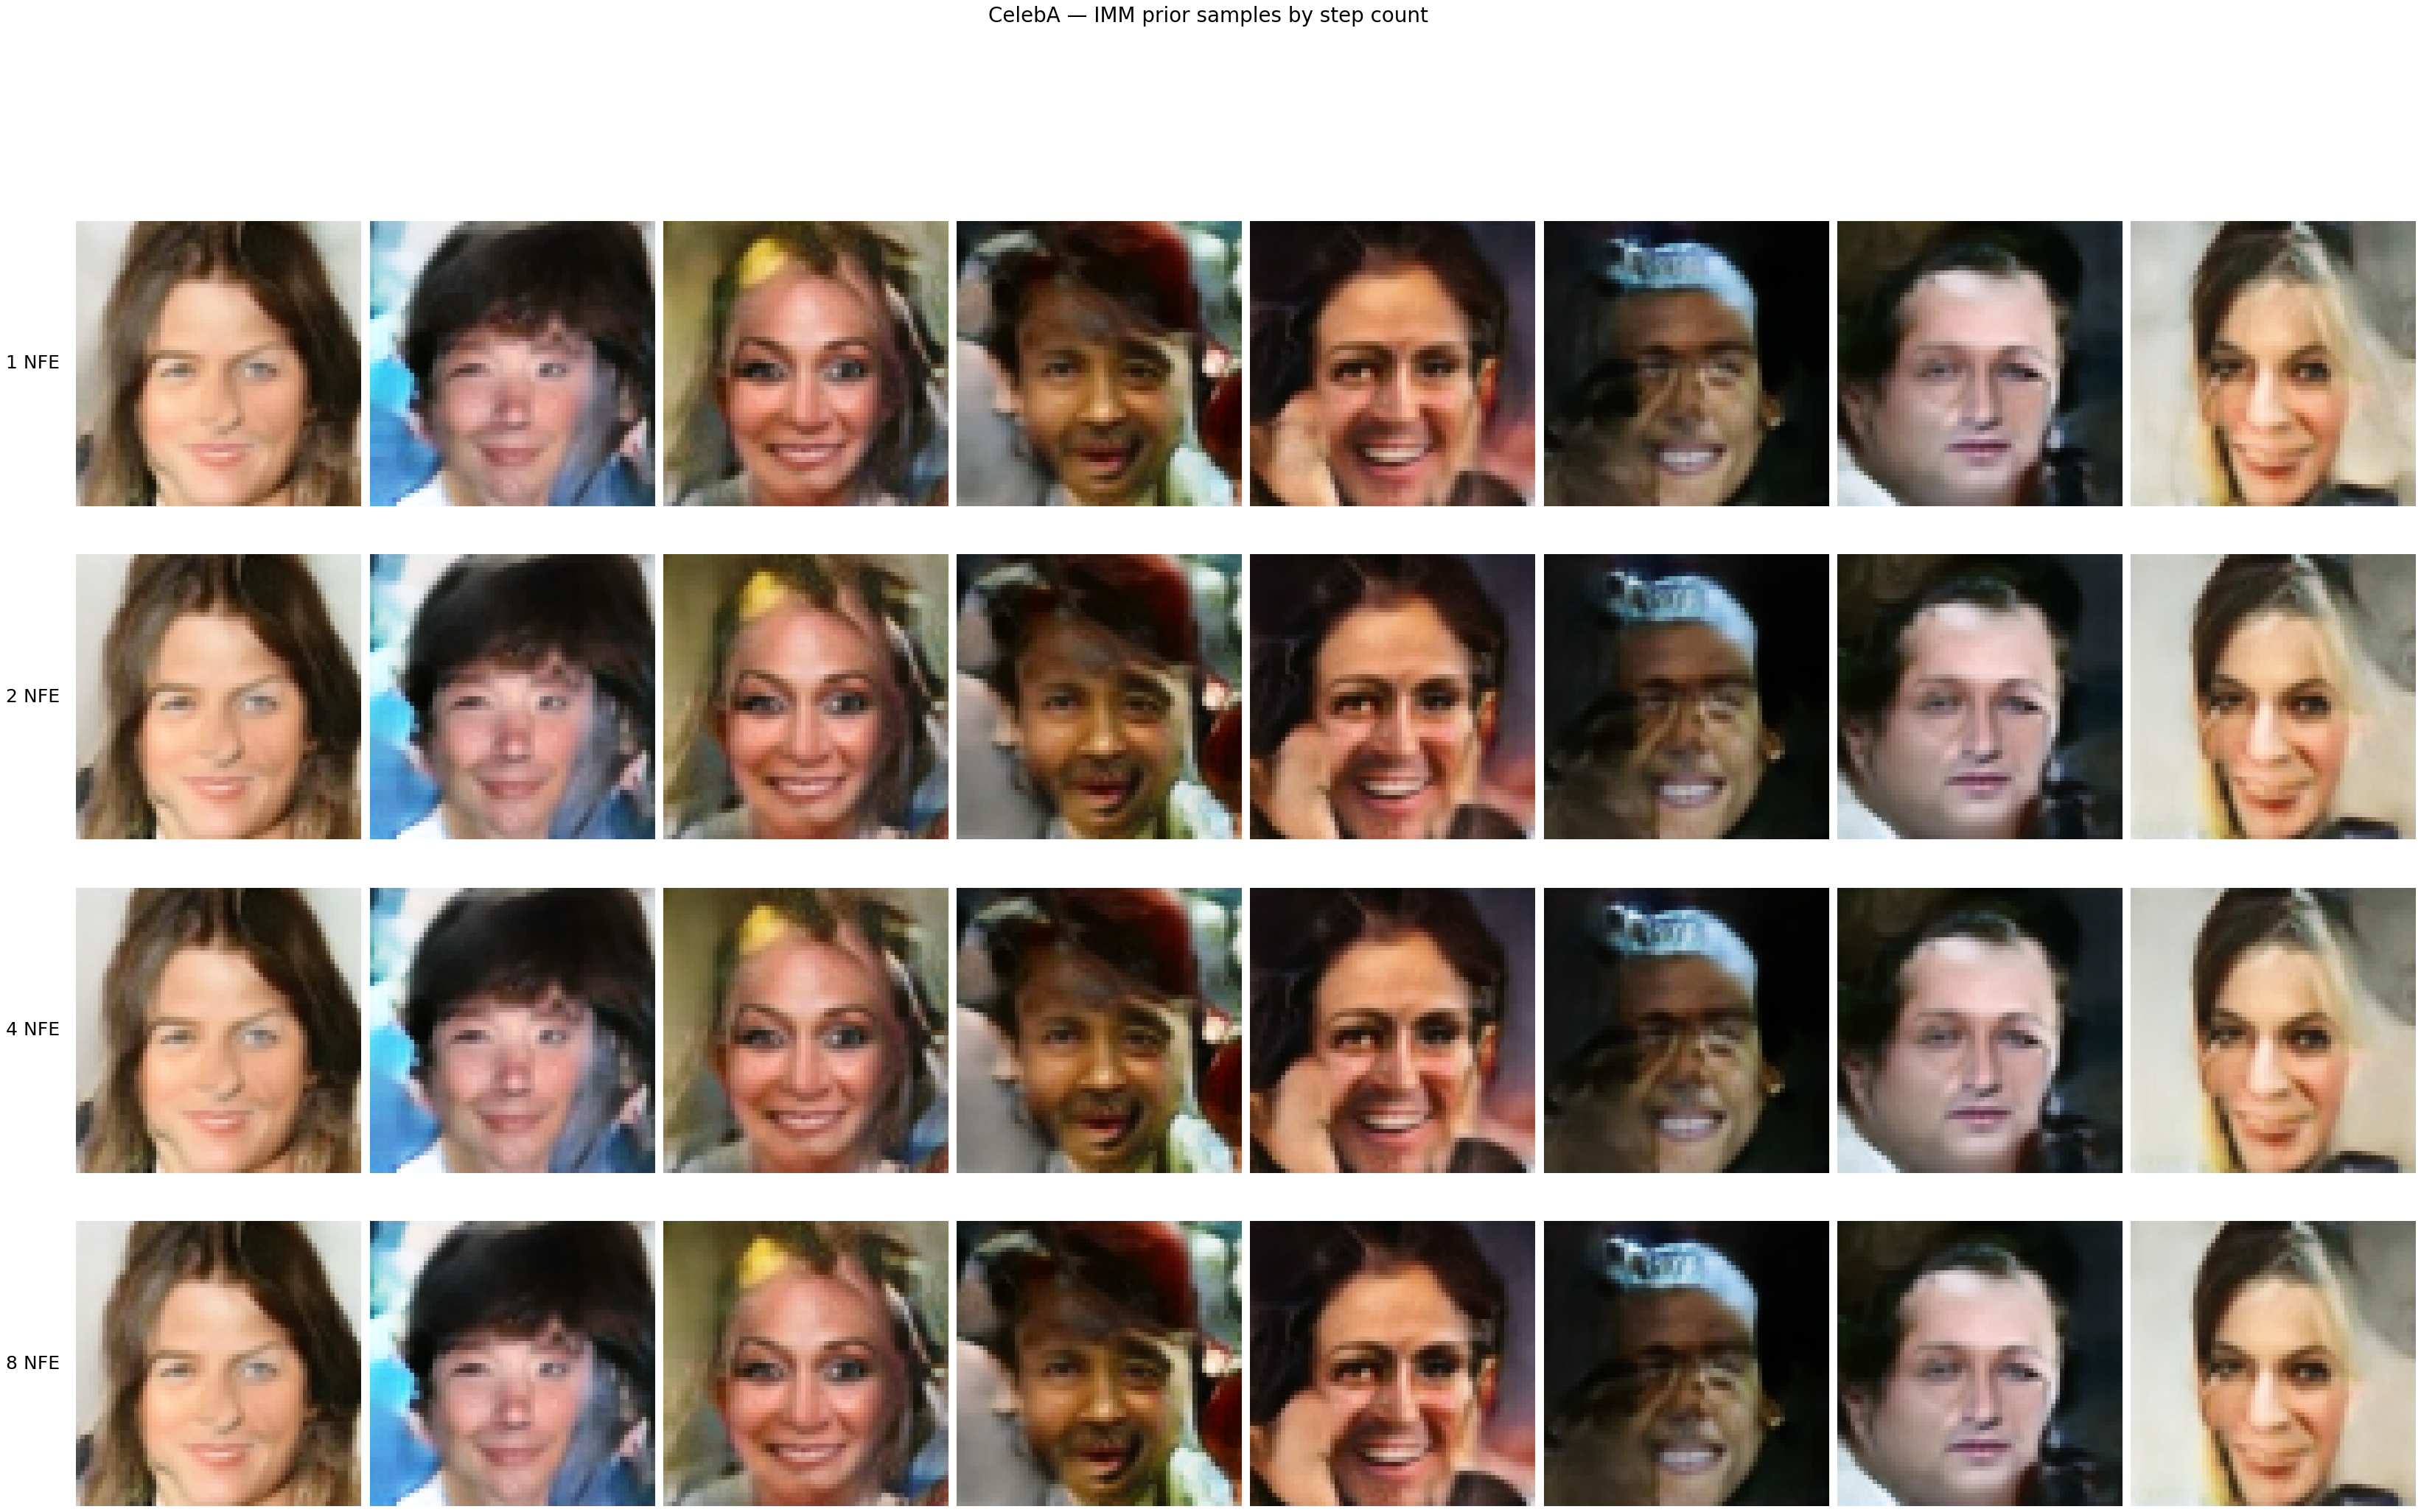
\includegraphics[width=\columnwidth]{figures/samples_CelebA64.png}
\caption{IMM prior samples by step count on the remaining settings. The
CelebA pattern (Figure~\ref{fig:samples}) --- most of the quality by $2$ NFE ---
holds on FFHQ, LSUN and CIFAR-10; ImageNet-32 keeps improving to $16$ NFE
($80.75 \to 75.85$).}
\label{fig:samples-rest}
\end{figure}

\section{Additional results}

\begin{table}[h]
\caption{Sampling grids provided with this submission.}
\begin{tabular}{ll}
\toprule
File & Contents \\
\midrule
\texttt{reconstructions\_*.png} & held-out reals (top) vs.\ reconstructions \\
\texttt{samples\_*.png}         & prior samples at 1, 2, 4, 8 NFE \\
\texttt{compare\_*.png}         & Gaussian / full-cov.\ / learned prior \\
\bottomrule
\end{tabular}
\end{table}

\end{document}
